\documentclass[11pt,letterpaper]{article}
\usepackage{fontspec}
\setmainfont{texgyrepagella}[Extension=.otf,UprightFont=*-regular,BoldFont=*-bold,ItalicFont=*-italic,BoldItalicFont=*-bolditalic]
\usepackage[bidi=default]{babel}
\babelprovide[import,main]{spanish}
\babelprovide[import]{hebrew}
\babelprovide[import]{ancientgreek}
\babelfont[hebrew]{rm}[Path=fonts/,BoldFont=NotoHebrewSerif-700.ttf,Scale=0.95]{NotoHebrewSerif-400.ttf}
\babelfont[ancientgreek]{rm}[Path=fonts/]{GFSPorson.otf}
\newcommand{\heb}[1]{\mbox{\foreignlanguage{hebrew}{#1}}}
\newcommand{\grc}[1]{\foreignlanguage{ancientgreek}{#1}}
\newcommand{\hebverso}[1]{\par\smallskip{\centering\begin{otherlanguage}{hebrew}\large #1\end{otherlanguage}\par}\smallskip}
\newcommand{\SENOR}{\textsc{Señor}}
\usepackage[margin=2.5cm,headheight=14pt]{geometry}
\usepackage{microtype,ragged2e,booktabs,graphicx,xcolor,csquotes,array}
\usepackage[hidelinks]{hyperref}\usepackage{xurl}\urlstyle{same}
\usepackage[most]{tcolorbox}
\usepackage{tikz}\usetikzlibrary{arrows.meta,positioning,calc,decorations.pathreplacing,shapes.geometric}
\usepackage{titlesec,fancyhdr}
\definecolor{tierraroja}{RGB}{122,40,18}\definecolor{caferojizo}{RGB}{58,18,8}
\definecolor{mostaza}{RGB}{214,160,58}\definecolor{papiro}{RGB}{243,228,192}\definecolor{sepia}{RGB}{98,66,44}
\definecolor{oliva}{RGB}{92,98,48}
\titleformat{\section}{\Large\bfseries\color{tierraroja}}{\thesection.}{0.6em}{}
\titleformat{\subsection}{\large\bfseries\color{caferojizo}}{\thesubsection}{0.6em}{}
\pagestyle{fancy}\fancyhf{}
\fancyhead[L]{\foreignlanguage{spanish}{\small\itshape\color{sepia}Shemitá}}\fancyhead[R]{\foreignlanguage{spanish}{\small\color{sepia}\thepage}}
\renewcommand{\headrulewidth}{0.4pt}
\setlength{\parindent}{1.27cm}\linespread{1.15}\setlength{\emergencystretch}{3em}
\newtcolorbox{cita}[1][]{enhanced,unbreakable,colback=tierraroja!5!white,colframe=tierraroja,boxrule=0pt,leftrule=2.5pt,arc=0pt,
  left=8pt,right=8pt,top=5pt,bottom=5pt,before skip=8pt,after skip=8pt,fontupper=\itshape,#1}
\newcommand{\fuente}[1]{\par\hfill{\upshape\bfseries\small\textcolor{tierraroja}{#1}}}
\newtcolorbox{nota}[1][]{enhanced,unbreakable,colback=mostaza!10,colframe=mostaza!85!tierraroja,boxrule=0.6pt,arc=2pt,
  fonttitle=\bfseries\small,coltitle=caferojizo,colbacktitle=mostaza!30,fontupper=\small,title={#1}}
\newtcolorbox{filologia}[1][]{enhanced,unbreakable,colback=white,colframe=tierraroja!45,boxrule=0.5pt,arc=2pt,
  fonttitle=\bfseries\small,coltitle=white,colbacktitle=tierraroja!80,fontupper=\small,title={Filología: #1}}
\newcommand{\refapa}[1]{\par{\RaggedRight\hangindent=1.27cm\hangafter=1\noindent #1\par}\vspace{4pt}}
\newcommand{\destacar}[1]{\textbf{\textcolor{tierraroja}{#1}}}
\newcolumntype{L}[1]{>{\RaggedRight\arraybackslash}p{#1}}

\title{\color{tierraroja}\bfseries Shemitá: el año sabático y el ciclo del siete\\[4pt]\large\color{sepia}\mdseries ``El séptimo año la tierra tendrá descanso, reposo para \SENOR'' (Lv 25:4)}
\author{}\date{}
\begin{document}
\maketitle\thispagestyle{empty}

\begin{abstract}\noindent
La Torá pide a un pueblo de campesinos algo que ninguna economía agraria se permite: dejar la tierra sin sembrar un año de cada siete, soltar al siervo hebreo con las manos llenas y remitir las deudas del hermano. La tradición llama a ese conjunto \emph{shemitá}, ``suelta'', por el verbo de Éx 23:11 y Dt 15:1--2. Este capítulo estudia la institución con el método de la serie. La lectura \emph{histórica} sitúa la ley en la economía de deuda y servidumbre del antiguo Cercano Oriente (los edictos babilonios de \emph{mīšarum}) y sigue su práctica atestiguada en el pacto de Nehemías, el asedio de Bet-sur (1~Mac 6), los decretos que recoge Josefo, el desprecio de Tácito, un pagaré de Murabba'at y el \emph{prosbul} de Hillel. La lectura \emph{filológica} recorre \emph{shamat}, \emph{shabatón}, \emph{sefiaj}, \emph{nazir}, \emph{derór}, \emph{ebyón} y \emph{nashá}, y sigue la cadena que considero más firme de todo el estudio: la Septuaginta traduce la ``suelta'' y la ``libertad'' con \grc{ἄφεσις}, la palabra con que el Nuevo Testamento nombra el perdón de los pecados y la remisión de las deudas (Lc 4:18; Mt 6:12; 26:28). La lectura \emph{textual} examina la sintaxis de Dt 15:2, la aparente tensión de Lv 25:5--6 y la cita compuesta de 2~Cr 36:21. La lectura \emph{literaria} ordena la escalera del siete (día, semana, mes, año, siete por siete años) y lee Lv 25--26 como unidad, con el exilio como el sábado que la tierra cobró. La síntesis recoge la lectura de la serie: el año séptimo prolonga el sábado de Lv 23:3 y apunta al reposo que queda para el pueblo de Dios (He 4:9).
\par\smallskip\noindent\textbf{Palabras clave:} shemitá, año sabático, Levítico 25, Deuteronomio 15, remisión, \emph{derór}, \grc{ἄφεσις}, reposo, setenta años.\end{abstract}

\begin{nota}[Nota sobre el texto]
Las citas bíblicas son de la Reina-Valera 1960 (RVR1960), convención de esta serie. Donde la RVR1960 escribe ``Jehová'', aquí se escribe \SENOR, que traduce el tetragrama \heb{יהוה}. Cuando una frase se traduce desde el original se indica ``(trad. propia)''. El hebreo sigue la BHS; el griego, NA28 y la Septuaginta de Rahlfs-Hanhart (citada como LXX). Las fuentes judías (Misná, Talmud, Rashi) se citan desde Sefaria y desde la traducción de Danby (1933), y se marcan como tradición posterior. Cuando la numeración hebrea difiere de la española se da entre corchetes, p.~ej. Neh 10:31 [10:32]. Las fechas son a.\,e.\,c. (antes de la era común) y e.\,c.; las del primer milenio son aproximadas. Los conteos de palabras son propios: se hicieron por lema (número de Strong) sobre el Códice de Leningrado etiquetado morfológicamente.
\end{nota}

%===================================================================
\section{Introducción: un año que no cabe en el calendario}

Levítico 23 abre el ``reglamento del culto'' con el sábado: ``Seis días se trabajará, mas el séptimo día será de reposo, santa convocación'' (Lv 23:3). Después vienen las siete fiestas del año, de Pésaj a Sukkot. La ley del siete, sin embargo, no termina en el séptimo día ni en el séptimo mes. Dos capítulos más adelante, en el mismo monte Sinaí (Lv 25:1), Dios extiende el sábado a la tierra:

\hebverso{וּבַשָּׁנָה הַשְּׁבִיעִת שַׁבַּת שַׁבָּתוֹן יִהְיֶה לָאָרֶץ שַׁבָּת לַיהוָה \\ שָׂדְךָ לֹא תִזְרָע וְכַרְמְךָ לֹא תִזְמֹר}
\begin{cita}Pero el séptimo año la tierra tendrá descanso, reposo para \SENOR; no sembrarás tu tierra, ni podarás tu viña.\fuente{(Lv 25:4)}\end{cita}

Antes que teológica, la pregunta que este texto vuelve urgente es práctica. ¿Qué come una familia campesina si no siembra? ¿Qué hace el acreedor cuando sabe que el préstamo se extinguirá en pocos meses? ¿Por qué un pueblo libre debería soltar a su siervo con regalos? La Torá formula esas mismas preguntas en voz alta, ``¿Qué comeremos el séptimo año?'' (Lv 25:20), ``Cerca está el año séptimo, el de la remisión'' (Dt 15:9), y las responde con una promesa y con un mandamiento.

Sostengo en este capítulo que la \emph{shemitá} es el \destacar{sábado de los años}. Prolonga el reposo del séptimo día hacia tres ámbitos que el sábado semanal no alcanza: la tierra, que descansa; el siervo hebreo, que sale libre; el deudor, cuya deuda se suelta. Las tres leyes nacen de una misma confesión, ``la tierra mía es'' (Lv 25:23), y de un mismo recuerdo, ``te acordarás de que fuiste siervo en la tierra de Egipto'' (Dt 15:15). Cuando Israel no guarda esos sábados, la Escritura los convierte en juicio, y la tierra ``gozará sus días de reposo'' durante el exilio (Lv 26:34; 2~Cr 36:21). Y cuando la Septuaginta traduce la ``suelta'' y la ``libertad'' con \grc{ἄφεσις}, deja preparada la palabra con que el Nuevo Testamento anunciará el perdón de los pecados.

El recorrido sigue el método de la serie: primero los textos (§2), con una tabla sinóptica; luego las lecturas histórica (§3), filológica (§4), textual (§5) y literaria (§6); después la lectura de la serie (§7), la shemitá en Jesús y los apóstoles (§8) y en la tradición judía (§9), la discusión de posturas (§10), la síntesis (§11) y las preguntas para la reflexión (§12).

Como la shemitá no es una de las siete fiestas de Lv 23, el esquema estándar de la serie no resalta ninguna. Su lugar está en el primer renglón del reglamento, el sábado, que Lv 25 proyecta sobre los años:

\begin{center}
% === Esquema estándar de la serie: el ciclo de Levítico 23 ===
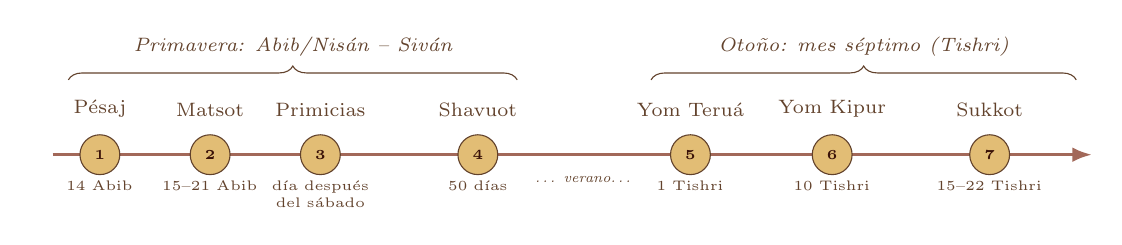
\begin{tikzpicture}[x=1cm,y=1cm,font=\scriptsize]
 \def\fiestaactual{0}
 \draw[line width=1.2pt,tierraroja!70,-{Latex[length=2.5mm]}] (0,0) -- (13.2,0);
 \draw[decorate,decoration={brace,amplitude=5pt},sepia] (0.2,0.95) -- (5.9,0.95) node[midway,above=5pt,font=\scriptsize\itshape]{Primavera: Abib/Nisán -- Siván};
 \draw[decorate,decoration={brace,amplitude=5pt},sepia] (7.6,0.95) -- (13.0,0.95) node[midway,above=5pt,font=\scriptsize\itshape]{Otoño: mes séptimo (Tishri)};
 \foreach \n/\x/\t/\d in {1/0.6/Pésaj/{14 Abib},2/2.0/Matsot/{15--21 Abib},3/3.4/Primicias/{día después del sábado},4/5.4/Shavuot/{50 días},5/8.1/Yom Teruá/{1 Tishri},6/9.9/Yom Kipur/{10 Tishri},7/11.9/Sukkot/{15--22 Tishri}}{
   \ifnum\n=\fiestaactual
     \node[circle,fill=tierraroja,draw=caferojizo,minimum size=5.5mm,text=papiro,font=\scriptsize\bfseries] at (\x,0) {\n};
     \node[above=3pt,font=\scriptsize\bfseries,text=tierraroja] at (\x,0.28) {\t};
   \else
     \node[circle,fill=mostaza!70,draw=sepia,minimum size=4.5mm,text=caferojizo,font=\tiny\bfseries] at (\x,0) {\n};
     \node[above=3pt,text=sepia] at (\x,0.25) {\t};
   \fi
   \node[below=6pt,text width=1.6cm,align=center,font=\tiny,text=sepia] at (\x,0) {\d};}
 \node[font=\tiny\itshape,text=sepia] at (6.75,-0.32) {\ldots\ verano\ldots};
\end{tikzpicture}\par
{\footnotesize\color{sepia}\textit{Figura 1.} El ciclo anual de Levítico 23. Ninguna fiesta se resalta: la shemitá no es un \emph{moed} del año, sino la extensión del sábado (Lv 23:3) a los años. \textit{Nota.} Esquema estándar de la serie.}
\end{center}

La figura siguiente muestra el ciclo propio de la shemitá. Así como el sábado semanal divide la semana en seis y uno, el año sabático divide del mismo modo la heptada de años: seis de trabajo y uno de reposo forman un ciclo, y siete ciclos llevan al año cincuenta, el jubileo, que se estudia en el capítulo siguiente (09, \emph{Jubileo}).

\begin{center}
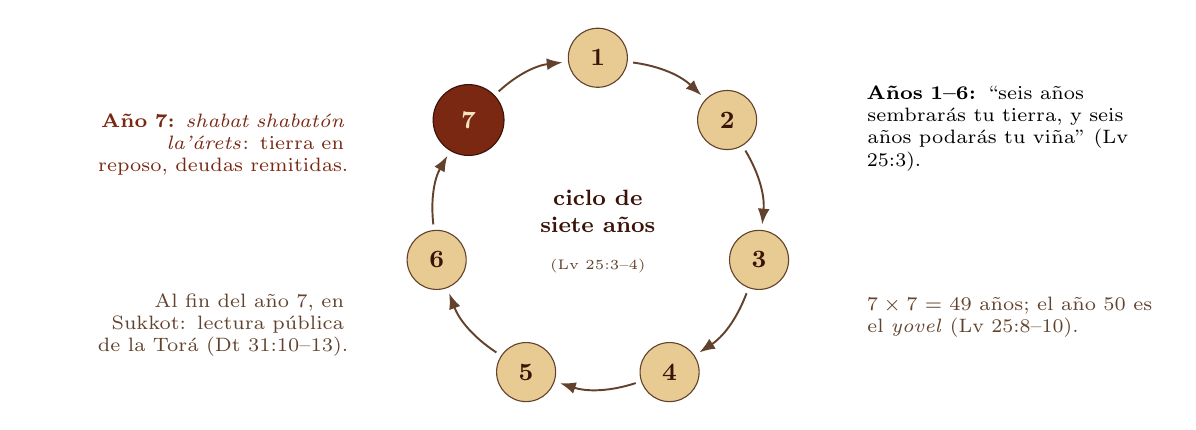
\begin{tikzpicture}[font=\scriptsize]
 \def\R{2.1}
 \foreach \i in {1,...,7}{
   \pgfmathsetmacro{\ang}{90-(\i-1)*360/7}
   \ifnum\i=7
     \node[circle,fill=tierraroja,text=papiro,draw=caferojizo,minimum size=9mm,font=\small\bfseries] (a\i) at (\ang:\R) {7};
   \else
     \node[circle,fill=mostaza!55,draw=sepia,minimum size=7.5mm,text=caferojizo,font=\small\bfseries] (a\i) at (\ang:\R) {\i};
   \fi}
 \foreach \i/\j in {1/2,2/3,3/4,4/5,5/6,6/7,7/1}{\draw[-{Latex[length=2mm]},sepia,line width=0.7pt,shorten >=2pt,shorten <=2pt] (a\i) to[bend left=18] (a\j);}
 \node[align=center,text=caferojizo,font=\footnotesize] at (0,0.15) {\textbf{ciclo de}\\\textbf{siete años}};
 \node[align=center,text=sepia,font=\tiny] at (0,-0.55) {(Lv 25:3--4)};
 \node[anchor=west,text width=3.7cm,font=\scriptsize] at (3.3,1.2) {\textbf{Años 1--6:} ``seis años sembrarás tu tierra, y seis años podarás tu viña'' (Lv 25:3).};
 \node[anchor=east,text width=3.9cm,align=right,font=\scriptsize,text=tierraroja] at (-3.1,1.0) {\textbf{Año 7:} \emph{shabat shabatón la'árets}: tierra en reposo, deudas remitidas.};
 \node[anchor=east,text width=3.9cm,align=right,font=\scriptsize,text=sepia] at (-3.1,-1.3) {Al fin del año 7, en Sukkot: lectura pública de la Torá (Dt 31:10--13).};
 \node[anchor=west,text width=3.7cm,font=\scriptsize,text=sepia] at (3.3,-1.2) {$7\times 7 = 49$ años; el año 50 es el \emph{yovel} (Lv 25:8--10).};
\end{tikzpicture}\par
{\footnotesize\color{sepia}\textit{Figura 2.} El ciclo de los años. \textit{Nota.} Elaboración propia con Lv 25:1--10 y Dt 15:1; 31:10. El año del siervo (Éx 21:2) se cuenta desde su compra, no desde este ciclo; véase §2.2.}
\end{center}

%===================================================================
\section{Los textos de la shemitá}

La ley del año séptimo aparece en los tres grandes cuerpos legales del Pentateuco: el Código de la Alianza (Éx 21--23), la Ley de Santidad (Lv 17--26) y el Deuteronomio (Dt 12--26), y cada uno la mira desde un ángulo distinto. Éxodo habla de la tierra y del siervo; Levítico, de la tierra como sujeto del sábado; Deuteronomio, del siervo y de las deudas. Los profetas y los libros históricos añaden la memoria de su incumplimiento.

\subsection{Éx 23:10--11: la tierra para los pobres}
El primer texto está en el calendario del Código de la Alianza, junto al sábado semanal (Éx 23:12) y las tres fiestas de peregrinación (23:14--17):

\hebverso{וְהַשְּׁבִיעִת תִּשְׁמְטֶנָּה וּנְטַשְׁתָּהּ וְאָכְלוּ אֶבְיֹנֵי עַמֶּךָ \\ וְיִתְרָם תֹּאכַל חַיַּת הַשָּׂדֶה כֵּן־תַּעֲשֶׂה לְכַרְמְךָ לְזֵיתֶךָ}
\begin{cita}Seis años sembrarás tu tierra, y recogerás su cosecha; mas el séptimo año la dejarás libre, para que coman los pobres de tu pueblo; y de lo que quedare comerán las bestias del campo; así harás con tu viña y con tu olivar.\fuente{(Éx 23:10--11)}\end{cita}

Dos verbos describen lo que el campesino hace en el año séptimo: \heb{תִּשְׁמְטֶנָּה} (\emph{tishmetenná}), ``la soltarás'', y \heb{וּנְטַשְׁתָּהּ} (\emph{unetashtah}), ``y la abandonarás''; la RVR1960 reúne ambos en ``la dejarás libre''. El primero da nombre a la institución; el segundo reaparecerá en el pacto de Nehemías (Neh 10:31 [10:32]). La finalidad está dicha en el propio versículo: que coman los \heb{אֶבְיֹנֵי עַמֶּךָ} (\emph{ebyoné ammeja}), ``los pobres de tu pueblo'', y después los animales salvajes. En Éxodo, por tanto, el año séptimo es ante todo una ley de asistencia, y las viñas y los olivares, cultivos de varios años, quedan incluidos: lo que no se poda ni se cosecha queda para otros.

\subsection{Éx 21:2--6 y Dt 15:12--18: el siervo hebreo}
La primera ley del Código de la Alianza, antes del homicidio y de las lesiones, es la del siervo:

\hebverso{כִּי תִקְנֶה עֶבֶד עִבְרִי שֵׁשׁ שָׁנִים יַעֲבֹד וּבַשְּׁבִעִת יֵצֵא לַחָפְשִׁי חִנָּם}
\begin{cita}Si comprares siervo hebreo, seis años servirá; mas al séptimo saldrá libre, de balde.\fuente{(Éx 21:2)}\end{cita}

El ``siervo hebreo'' es aquí, con toda probabilidad, un israelita que se vendió o fue vendido por deudas, y el texto pone a su servicio un límite de seis años. En el séptimo sale \heb{לַחָפְשִׁי} (\emph{lajofshí}), ``a la libertad'', y \heb{חִנָּם} (\emph{jinnam}), ``gratis'', sin pagar rescate. Si el siervo prefiere quedarse (``Yo amo a mi señor, a mi mujer y a mis hijos, no saldré libre''), su amo le horada la oreja con lesna junto a la puerta, ``y será su siervo para siempre'' (Éx 21:5--6). La ley prevé el afecto, pero lo hace público y excepcional.

Deuteronomio retoma la ley y la amplía: incluye a la mujer (``tu hermano hebreo o hebrea''), llama al siervo ``tu hermano'' y prohíbe despedirlo con las manos vacías:

\hebverso{וְכִי־תְשַׁלְּחֶנּוּ חָפְשִׁי מֵעִמָּךְ לֹא תְשַׁלְּחֶנּוּ רֵיקָם \\ הַעֲנֵיק תַּעֲנִיק לוֹ מִצֹּאנְךָ וּמִגָּרְנְךָ וּמִיִּקְבֶךָ}
\begin{cita}Si se vendiere a ti tu hermano hebreo o hebrea, y te hubiere servido seis años, al séptimo le despedirás libre. Y cuando lo despidieres libre, no le enviarás con las manos vacías. Le abastecerás liberalmente de tus ovejas, de tu era y de tu lagar; le darás de aquello en que \SENOR{} te hubiere bendecido. Y te acordarás de que fuiste siervo en la tierra de Egipto, y que \SENOR{} tu Dios te rescató; por tanto yo te mando esto hoy.\fuente{(Dt 15:12--15)}\end{cita}

``Le abastecerás liberalmente'' traduce \heb{הַעֲנֵיק תַּעֲנִיק} (\emph{haaneq taaniq}), un verbo raro emparentado con \emph{anaq}, ``collar'': ``le pondrás un collar'', ``le cargarás el cuello'' de regalos (BDB; Tigay, 1996). El siervo sale con un capital para empezar de nuevo, ovejas, grano de la era, vino del lagar. La motivación es un memorial, \heb{וְזָכַרְתָּ כִּי עֶבֶד הָיִיתָ} (\emph{vezajartá ki éved hayita}), ``y te acordarás de que fuiste siervo'': Israel salió de Egipto con las manos llenas (Éx 3:21--22; 12:35--36), y el siervo hebreo debe salir del mismo modo. El texto termina previendo la resistencia del amo: ``No te parezca duro cuando le enviares libre, pues por la mitad del costo de un jornalero te sirvió seis años'' (Dt 15:18; sobre esta frase, véase §5).

\begin{nota}[Precisión]
El año de libertad del siervo (Éx 21:2; Dt 15:12) se cuenta desde que comenzó su servicio: ``seis años servirá''. No coincide necesariamente con el año sabático de la tierra (Lv 25:4) ni con el año de remisión de las deudas (Dt 15:1), que son fechas fijas para todo el país. La tradición rabínica trata la salida del siervo hebreo ``por años'' como un cómputo propio (Misná \emph{Kidushín} 1:2). Jer 34 parece reunir ambos cómputos en una liberación general y simultánea (véase §2.8). La relación entre el siervo de Éx 21 y Dt 15 y la ley del jubileo de Lv 25:39--46 se estudia en el capítulo 09.
\end{nota}

\subsection{Lv 25:1--7: la tierra guarda sábado}
Levítico da a la institución su formulación más teológica, con la tierra como sujeto del sábado:

\hebverso{כִּי תָבֹאוּ אֶל־הָאָרֶץ אֲשֶׁר אֲנִי נֹתֵן לָכֶם וְשָׁבְתָה הָאָרֶץ שַׁבָּת לַיהוָה}
\begin{cita}\SENOR{} habló a Moisés en el monte de Sinaí, diciendo: Habla a los hijos de Israel y diles: Cuando hayáis entrado en la tierra que yo os doy, la tierra guardará reposo para \SENOR. Seis años sembrarás tu tierra, y seis años podarás tu viña y recogerás sus frutos. Pero el séptimo año la tierra tendrá descanso, reposo para \SENOR; no sembrarás tu tierra, ni podarás tu viña.\fuente{(Lv 25:1--4)}\end{cita}

El verbo de v.~2 es \heb{וְשָׁבְתָה} (\emph{veshavtá}), ``y descansará'', ``y guardará sábado''. El año séptimo recibe el mismo título que el sábado semanal (Éx 31:15; 35:2; Lv 23:3) y que el Día de la Expiación (Lv 16:31; 23:32), \heb{שַׁבַּת שַׁבָּתוֹן} (\emph{shabat shabatón}), ``sábado de reposo solemne'', y la frase \heb{שַׁבָּת לַיהוָה} (\emph{shabat laYHWH}), ``sábado para el \SENOR'', es la del cuarto mandamiento (Éx 20:10; Dt 5:14). Con ese vocabulario, el sábado de la tierra queda definido como tiempo consagrado y no como mera técnica de barbecho.

La ley se aplica desde la entrada, ``cuando hayáis entrado en la tierra'' (v.~2). Volveremos sobre esta cláusula en la lectura de la serie (§7), porque supone a Israel ya establecido en Canaán, el hito que la serie asocia con Josué y con el reposo.

\begin{cita}Lo que de suyo naciere en tu tierra segada, no lo segarás, y las uvas de tu viñedo no vendimiarás; año de reposo será para la tierra. Mas el descanso de la tierra te dará para comer a ti, a tu siervo, a tu sierva, a tu criado, y a tu extranjero que morare contigo; y a tu animal, y a la bestia que hubiere en tu tierra, será todo el fruto de ella para comer.\fuente{(Lv 25:5--7)}\end{cita}

Lo que crece solo, \heb{סְפִיחַ} (\emph{sefiaj}), no se siega como cosecha, pero alimenta a todos: al dueño, al siervo, a la sierva, al jornalero, al residente extranjero, al ganado y a los animales salvajes. Donde Éxodo daba el año a los pobres, Levítico lo da a todos por igual, de modo que en el año séptimo desaparece la diferencia entre el dueño que cosecha y el pobre que espiga; todos comen del campo como huéspedes del \SENOR. La lista de v.~6 se parece a la del mandamiento del sábado (Éx 20:10; Dt 5:14).

\subsection{Lv 25:18--22: ``¿Qué comeremos?''}
Después de la ley del jubileo, Levítico vuelve al año séptimo y formula la objeción del campesino:

\hebverso{וְכִי תֹאמְרוּ מַה־נֹּאכַל בַּשָּׁנָה הַשְּׁבִיעִת הֵן לֹא נִזְרָע וְלֹא נֶאֱסֹף אֶת־תְּבוּאָתֵנוּ \\ וְצִוִּיתִי אֶת־בִּרְכָתִי לָכֶם בַּשָּׁנָה הַשִּׁשִּׁית וְעָשָׂת אֶת־הַתְּבוּאָה לִשְׁלֹשׁ הַשָּׁנִים}
\begin{cita}Y si dijereis: ¿Qué comeremos el séptimo año? He aquí no hemos de sembrar, ni hemos de recoger nuestros frutos; entonces yo os enviaré mi bendición el sexto año, y ella hará que haya fruto por tres años. Y sembraréis el año octavo, y comeréis del fruto añejo; hasta el año noveno, hasta que venga su fruto, comeréis del añejo.\fuente{(Lv 25:20--22)}\end{cita}

``Os enviaré mi bendición'' es, literalmente, \heb{וְצִוִּיתִי אֶת־בִּרְכָתִי} (\emph{vetsiviti et birjatí}), ``mandaré mi bendición'': la bendición obedece una orden, como un siervo enviado. La lógica es la del maná, cuando el sexto día caía doble porción para el sábado (Éx 16:22--29). El texto no exige un heroísmo sin red, sino que promete una cosecha triple que cubre el año sexto, el séptimo y el octavo, hasta que llegue la cosecha nueva. La condición la fija v.~18, ``Ejecutad, pues, mis estatutos y guardad mis ordenanzas, y ponedlos por obra, y habitaréis en la tierra seguros'': la seguridad en la tierra depende de confiar en su Dueño.

\begin{center}
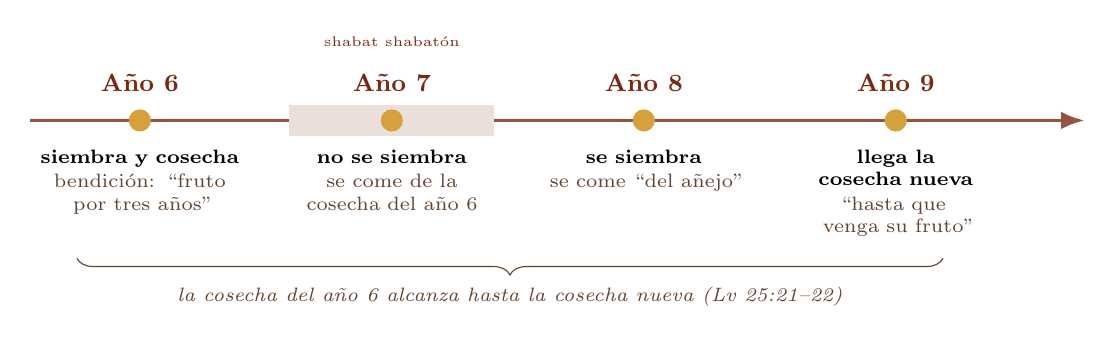
\begin{tikzpicture}[font=\scriptsize]
 \draw[line width=1.4pt,tierraroja!80,-{Latex[length=3mm]}] (0,0) -- (13.4,0);
 \fill[tierraroja!15] (3.3,-0.2) rectangle (5.9,0.2);
 \foreach \x/\a/\b/\c in {1.4/{Año 6}/{siembra y cosecha}/{bendición: ``fruto por tres años''},4.6/{Año 7}/{no se siembra}/{se come de la cosecha del año 6},7.8/{Año 8}/{se siembra}/{se come ``del añejo''},11.0/{Año 9}/{llega la cosecha nueva}/{``hasta que venga su fruto''}}{
   \fill[mostaza] (\x,0) circle (4pt);
   \node[above=7pt,font=\small\bfseries,text=tierraroja] at (\x,0) {\a};
   \node[below=7pt,text width=2.6cm,align=center,font=\scriptsize] at (\x,0) {\textbf{\b}\\[1pt] {\color{sepia}\c}};}
 \node[font=\tiny\itshape,text=tierraroja] at (4.6,1.0) {\emph{shabat shabatón}};
 \draw[decorate,decoration={brace,amplitude=6pt,mirror},sepia] (0.6,-1.75) -- (11.6,-1.75) node[midway,below=7pt,font=\scriptsize\itshape,text=sepia] {la cosecha del año 6 alcanza hasta la cosecha nueva (Lv 25:21--22)};
\end{tikzpicture}\par
{\footnotesize\color{sepia}\textit{Figura 3.} La cosecha triple del año sexto. \textit{Nota.} Elaboración propia con Lv 25:20--22. El cómputo exacto depende de si el año agrícola se cuenta desde el otoño; véase §5.}
\end{center}

\subsection{Dt 15:1--11: la remisión de las deudas}
Deuteronomio llama al año séptimo con el sustantivo que le dará nombre: \emph{shemitá}.

\hebverso{מִקֵּץ שֶׁבַע־שָׁנִים תַּעֲשֶׂה שְׁמִטָּה \\ וְזֶה דְּבַר הַשְּׁמִטָּה שָׁמוֹט כָּל־בַּעַל מַשֵּׁה יָדוֹ אֲשֶׁר יַשֶּׁה בְּרֵעֵהוּ \\ לֹא־יִגֹּשׂ אֶת־רֵעֵהוּ וְאֶת־אָחִיו כִּי־קָרָא שְׁמִטָּה לַיהוָה}
\begin{cita}Cada siete años harás remisión. Y esta es la manera de la remisión: perdonará a su deudor todo aquel que hizo empréstito de su mano, con el cual obligó a su prójimo; no lo demandará más a su prójimo, o a su hermano, porque es pregonada la remisión de \SENOR.\fuente{(Dt 15:1--2)}\end{cita}

La remisión es ``de \SENOR'', \heb{שְׁמִטָּה לַיהוָה} (\emph{shemitá laYHWH}), con la misma preposición que el ``sábado para el \SENOR'' de Lv 25:2, 4. El verbo \emph{qará}, ``proclamar'', indica un acto público: la remisión se pregona, como el jubileo (Lv 25:10) y las convocaciones (Lv 23:2). La ley protege al ``prójimo'' y al ``hermano'', y excluye al \heb{נָכְרִי} (\emph{nojrí}), el extranjero de paso, que presta y toma prestado por comercio: ``Del extranjero demandarás el reintegro; pero lo que tu hermano tuviere tuyo, lo perdonará tu mano'' (v.~3).

El pasaje contiene una tensión que el propio legislador parece haber buscado:

\hebverso{אֶפֶס כִּי לֹא יִהְיֶה־בְּךָ אֶבְיוֹן \foreignlanguage{spanish}{[\ldots]} \\ כִּי לֹא־יֶחְדַּל אֶבְיוֹן מִקֶּרֶב הָאָרֶץ}
\begin{cita}para que así no haya en medio de ti mendigo; porque \SENOR{} te bendecirá con abundancia en la tierra que \SENOR{} tu Dios te da por heredad para que la tomes en posesión\ldots\fuente{(Dt 15:4)}\end{cita}
\begin{cita}Porque no faltarán menesterosos en medio de la tierra; por eso yo te mando, diciendo: Abrirás tu mano a tu hermano, al pobre y al menesteroso en tu tierra.\fuente{(Dt 15:11)}\end{cita}

La misma palabra, \heb{אֶבְיוֹן} (\emph{ebyón}), aparece en ambos versos; la RVR1960 la traduce ``mendigo'' en v.~4 y ``menesterosos'' en v.~11. Leídos por separado parecen contradecirse (no habrá pobres; siempre habrá pobres), pero en su contexto describen dos horizontes. El v.~4 dice lo que ocurriría si Israel obedeciera plenamente (vv.~5--6: ``si escuchares fielmente la voz de \SENOR''); el v.~11 dice lo que ocurrirá de hecho en una sociedad real, y por eso manda ``abrirás tu mano''. La promesa no exime del mandato, y el realismo no anula la promesa (Tigay, 1996; Hamilton, 1992). Jesús citará la segunda frase, ``siempre tendréis pobres con vosotros'' (Mt 26:11), y Marcos añade ``y cuando queráis les podréis hacer bien'' (Mr 14:7).

El v.~9 nombra la tentación que la ley prevé:

\hebverso{הִשָּׁמֶר לְךָ פֶּן־יִהְיֶה דָבָר עִם־לְבָבְךָ בְלִיַּעַל לֵאמֹר \\ קָרְבָה שְׁנַת־הַשֶּׁבַע שְׁנַת הַשְּׁמִטָּה וְרָעָה עֵינְךָ בְּאָחִיךָ הָאֶבְיוֹן}
\begin{cita}Guárdate de tener en tu corazón pensamiento perverso, diciendo: Cerca está el año séptimo, el de la remisión, y mires con malos ojos a tu hermano menesteroso para no darle; porque él podrá clamar contra ti a \SENOR, y se te contará por pecado.\fuente{(Dt 15:9)}\end{cita}

``Pensamiento perverso'' es, literalmente, ``una palabra con tu corazón, de \emph{beliyaal}''. El término \heb{בְּלִיַּעַל} designa lo que no vale nada y destruye; los ``hombres impíos'' de Dt 13:13 [13:14] son ``hijos de \emph{beliyaal}'', y en la literatura del Segundo Templo y en Pablo, Belial pasa a ser nombre del adversario (2~Co 6:15). Aquí describe un cálculo económico frío, el de no prestar porque la remisión está cerca. Deuteronomio llama a ese cálculo ``de Belial'' y lo convierte en pecado, porque el pobre ``podrá clamar contra ti'', con el verbo del clamor de Israel en Egipto (Éx 3:7, 9). Que la tentación era real lo mostrará la historia posterior (véase el \emph{prosbul}, §9).

\subsection{Dt 31:9--13: la Torá leída en el año de la remisión}
El año de la remisión termina con un acto litúrgico:

\hebverso{מִקֵּץ שֶׁבַע שָׁנִים בְּמֹעֵד שְׁנַת הַשְּׁמִטָּה בְּחַג הַסֻּכּוֹת}
\begin{cita}Y les mandó Moisés, diciendo: Al fin de cada siete años, en el año de la remisión, en la fiesta de los tabernáculos, cuando viniere todo Israel a presentarse delante de \SENOR{} tu Dios en el lugar que él escogiere, leerás esta ley delante de todo Israel a oídos de ellos. Harás congregar al pueblo, varones y mujeres y niños, y tus extranjeros que estuvieren en tus ciudades, para que oigan y aprendan, y teman a \SENOR{} vuestro Dios, y cuiden de cumplir todas las palabras de esta ley.\fuente{(Dt 31:10--12)}\end{cita}

La tradición llama a esta asamblea \heb{הַקְהֵל} (\emph{haqhel}), por el imperativo de v.~12, ``congrega''. El texto une la shemitá con Sukkot, la última fiesta del ciclo de Lv 23, y con la Torá: el año en que la tierra descansó y las deudas se soltaron se cierra con la lectura pública de la ley, y el pueblo liberado vuelve a oír los términos de su pacto. La expresión ``en el \emph{moed} del año de la remisión'' (\heb{בְּמֹעֵד}) usa la palabra de Lv 23:2, ``las fiestas solemnes''.

\subsection{Lv 26:34--35, 43 y 2~Cr 36:20--21: la tierra cobra sus sábados}
La sección de bendiciones y maldiciones que cierra el Código de Santidad (Lv 26) incluye una amenaza que solo tiene sentido después de Lv 25:

\hebverso{אָז תִּרְצֶה הָאָרֶץ אֶת־שַׁבְּתֹתֶיהָ כֹּל יְמֵי הֳשַׁמָּה וְאַתֶּם בְּאֶרֶץ אֹיְבֵיכֶם \\ אָז תִּשְׁבַּת הָאָרֶץ וְהִרְצָת אֶת־שַׁבְּתֹתֶיהָ}
\begin{cita}Entonces la tierra gozará sus días de reposo, todos los días que esté asolada, mientras vosotros estéis en la tierra de vuestros enemigos; la tierra descansará entonces y gozará sus días de reposo. Todo el tiempo que esté asolada, descansará por lo que no reposó en los días de reposo cuando habitabais en ella.\fuente{(Lv 26:34--35)}\end{cita}

``Gozará'' traduce \heb{תִּרְצֶה} (\emph{tirtsé}), del verbo \emph{ratsá}, ``aceptar, complacerse, saldar''. La forma causativa de v.~34b, \heb{וְהִרְצָת}, suele entenderse como ``saldará'', ``cobrará'': la tierra recibe como pago los sábados que se le negaron (Milgrom, 2001; Hartley, 1992), y el exilio queda descrito como una deuda que se cobra en tiempo. El v.~43 lo repite: ``la tierra será abandonada por ellos, y gozará sus días de reposo, estando desierta a causa de ellos''. Hay además un juego sonoro en estos versos: \heb{הֳשַׁמָּה} (\emph{hoshammá}, ``la desolación'', raíz \emph{shamam}) suena cerca de \emph{shemitá} (raíz \emph{shamat}), y \heb{בְּשִׁבְתְּכֶם} (\emph{beshivtejem}, ``cuando habitabais'', raíz \emph{yashav}) suena cerca de \emph{shabat}.

El cronista lee la caída de Jerusalén con este texto:

\hebverso{לְמַלֹּאות דְּבַר־יְהוָה בְּפִי יִרְמְיָהוּ עַד־רָצְתָה הָאָרֶץ אֶת־שַׁבְּתוֹתֶיהָ \\ כָּל־יְמֵי הָשַּׁמָּה שָׁבָתָה לְמַלֹּאות שִׁבְעִים שָׁנָה}
\begin{cita}Los que escaparon de la espada fueron llevados cautivos a Babilonia, y fueron siervos de él y de sus hijos, hasta que vino el reino de los persas; para que se cumpliese la palabra de \SENOR{} por boca de Jeremías, hasta que la tierra hubo gozado de reposo; porque todo el tiempo de su asolamiento reposó, hasta que los setenta años fueron cumplidos.\fuente{(2~Cr 36:20--21)}\end{cita}

El cronista une dos profecías. De Jeremías toma los setenta años (``servirán estas naciones al rey de Babilonia setenta años'', Jer 25:11; ``Cuando en Babilonia se cumplan los setenta años, yo os visitaré'', Jer 29:10); de Levítico, la tierra que ``goza sus sábados''. No se le escapa la ironía: los que no soltaron a sus siervos ``fueron siervos'' en Babilonia. La relación numérica entre setenta años y años sabáticos incumplidos se discute en §3.5 y §5.

\subsection{Jer 34:8--22: la libertad revocada}
El único relato bíblico de una liberación de siervos ocurre durante el asedio babilónico de Jerusalén (ca.~588 a.\,e.\,c.). El rey Sedequías hace un pacto con el pueblo ``para promulgarles libertad'', \heb{לִקְרֹא לָהֶם דְּרוֹר} (\emph{liqró lahem derór}, Jer 34:8). Todos sueltan a sus siervos y siervas hebreos; ``pero después se arrepintieron, e hicieron volver a los siervos y a las siervas que habían dejado libres, y los sujetaron como siervos y siervas'' (v.~11). El contexto sugiere la causa: el ejército babilonio levantó el sitio por un tiempo ante la llegada de los egipcios (Jer 34:21--22; 37:5--11), y el peligro pareció pasar.

Dios recuerda la ley (``Al cabo de siete años dejará cada uno a su hermano hebreo que le fuere vendido; le servirá seis años, y lo enviará libre'', v.~14, que combina Dt 15:1 y 15:12) y responde con una justicia en espejo:

\hebverso{הִנְנִי קֹרֵא לָכֶם דְּרוֹר נְאֻם־יְהוָה אֶל־הַחֶרֶב אֶל־הַדֶּבֶר וְאֶל־הָרָעָב}
\begin{cita}Por tanto, así ha dicho \SENOR: Vosotros no me habéis oído para promulgar cada uno libertad a su hermano, y cada uno a su compañero; he aquí que yo promulgo libertad, dice \SENOR, a la espada y a la pestilencia y al hambre; y os pondré por afrenta ante todos los reinos de la tierra.\fuente{(Jer 34:17)}\end{cita}

La palabra \emph{derór} aparece en el relato cuatro veces (vv.~8, 15 y dos en v.~17; conteo propio). Ellos ``proclamaron libertad'' y la revocaron; Dios ``proclama libertad'' a la espada, que queda ``suelta'' contra el pueblo que no soltó a sus hermanos. El castigo reproduce así la forma del pecado. El relato añade el rito del pacto: los príncipes pasaron entre las mitades de un becerro partido (vv.~18--19; cf. Gn 15:9--17), y por eso serán entregados como el becerro.

\begin{center}
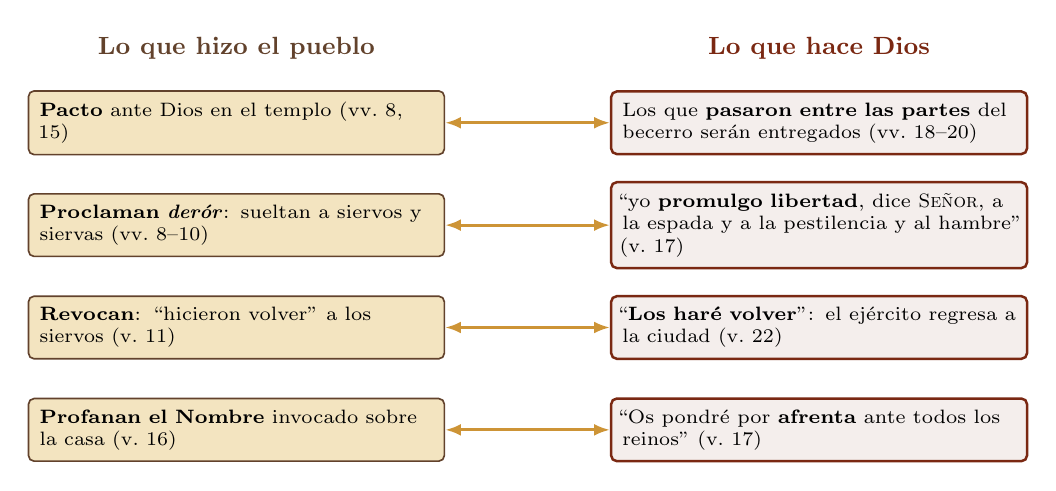
\begin{tikzpicture}[font=\scriptsize,
  izq/.style={draw=sepia,line width=0.6pt,fill=papiro,rounded corners=2pt,text width=5.0cm,align=left,inner sep=4pt},
  der/.style={draw=tierraroja,line width=0.9pt,fill=tierraroja!8,rounded corners=2pt,text width=5.0cm,align=left,inner sep=4pt}]
 \node[font=\small\bfseries,text=sepia] at (0,4.25) {Lo que hizo el pueblo};
 \node[font=\small\bfseries,text=tierraroja] at (7.4,4.25) {Lo que hace Dios};
 \node[izq] (a1) at (0,3.3) {\textbf{Pacto} ante Dios en el templo (vv.~8, 15)};
 \node[izq] (a2) at (0,2.0) {\textbf{Proclaman \emph{derór}}: sueltan a siervos y siervas (vv.~8--10)};
 \node[izq] (a3) at (0,0.7) {\textbf{Revocan}: ``hicieron volver'' a los siervos (v.~11)};
 \node[izq] (a4) at (0,-0.6) {\textbf{Profanan el Nombre} invocado sobre la casa (v.~16)};
 \node[der] (b1) at (7.4,3.3) {Los que \textbf{pasaron entre las partes} del becerro serán entregados (vv.~18--20)};
 \node[der] (b2) at (7.4,2.0) {``yo \textbf{promulgo libertad}, dice \SENOR, a la espada y a la pestilencia y al hambre'' (v.~17)};
 \node[der] (b3) at (7.4,0.7) {``\textbf{Los haré volver}'': el ejército regresa a la ciudad (v.~22)};
 \node[der] (b4) at (7.4,-0.6) {``Os pondré por \textbf{afrenta} ante todos los reinos'' (v.~17)};
 \foreach \i in {1,2,3,4}{\draw[{Latex[length=2mm]}-{Latex[length=2mm]},mostaza!90!tierraroja,line width=1pt] (a\i.east) -- (b\i.west);}
\end{tikzpicture}\par
{\footnotesize\color{sepia}\textit{Figura 4.} Jer 34: la libertad revocada y la libertad ``a la espada''. \textit{Nota.} Elaboración propia con Jer 34:8--22 (RVR1960). En v.~22 el hebreo usa el mismo verbo \emph{shuv} (``hacer volver'') de v.~11.}
\end{center}

\subsection{Neh 10:31 [10:32]: el pacto de los que volvieron}
Después del exilio, la comunidad de Jerusalén firma un pacto escrito. Entre sus cláusulas está el año séptimo:

\hebverso{וְנִטֹּשׁ אֶת־הַשָּׁנָה הַשְּׁבִיעִית וּמַשָּׁא כָל־יָד}
\begin{cita}asimismo, que si los pueblos de la tierra trajesen a vender mercaderías y comestibles en día de reposo, nada tomaríamos de ellos en ese día ni en otro día santificado; y que el año séptimo dejaríamos descansar la tierra, y remitiríamos toda deuda.\fuente{(Neh 10:31 [10:32])}\end{cita}

La cláusula une en una sola frase el verbo de Éx 23:11 (\heb{נָטַשׁ}, \emph{natash}, ``abandonar'' la tierra) y el vocabulario de Dt 15:2 (\heb{מַשָּׁא יָד}, \emph{mashá yad}, ``el préstamo de la mano''). Tenemos aquí un ejemplo temprano de lectura conjunta de la Torá, pues los que volvieron del exilio leen Éxodo y Deuteronomio como una sola ley. Y como la cláusula sigue inmediatamente a la del sábado, la comunidad parece entender el año séptimo como extensión del séptimo día.

\subsection{Tabla sinóptica}

\begin{center}\footnotesize\renewcommand{\arraystretch}{1.12}
\begin{tabular}{@{}L{2.3cm}L{1.9cm}L{6.2cm}L{3.9cm}@{}}
\toprule
\textbf{Texto} & \textbf{Ámbito} & \textbf{Qué añade} & \textbf{Motivación} \\ \midrule
Éx 21:2--6 & siervo & límite de seis años; sale ``libre, de balde''; la oreja horadada si elige quedarse & --- (ley de casos) \\
Éx 23:10--11 & tierra & la tierra ``soltada'' y ``abandonada''; viñas y olivos incluidos & que coman los pobres y las bestias \\
Lv 25:1--7 & tierra & la tierra es sujeto: \emph{shabat shabatón}, \emph{shabat laYHWH}; no sembrar ni podar; el \emph{sefiaj} para todos & el sábado del \SENOR{} \\
Lv 25:18--22 & tierra & la objeción ``¿qué comeremos?'' y la cosecha triple & la bendición mandada \\
Lv 26:34--35, 43 & tierra & el exilio como sábados cobrados & la desobediencia \\
Dt 15:1--11 & deudas & \emph{shemitá} pregonada; remisión al hermano, no al extranjero; tensión vv.~4/11; el pensamiento ``de Belial'' & ``que así no haya en medio de ti mendigo''; la bendición \\
Dt 15:12--18 & siervo & incluye a la hebrea; ``tu hermano''; provisión generosa & ``fuiste siervo en Egipto'' \\
Dt 31:9--13 & culto & lectura de la Torá en Sukkot del año de la remisión (\emph{haqhel}) & que oigan, aprendan y teman \\
Jer 34:8--22 & siervo & \emph{derór} proclamado y revocado; libertad ``a la espada'' & el pacto con los padres \\
2~Cr 36:20--21 & tierra & los setenta años como reposo de la tierra & la palabra de Jeremías \\
Neh 10:31 [10:32] & tierra, deudas & pacto escrito que une Éx 23 y Dt 15 & renovación del pacto \\
\bottomrule
\end{tabular}\par
{\footnotesize\color{sepia}\textit{Tabla 1.} Los textos del año séptimo. \textit{Nota.} Elaboración propia con la RVR1960 y la BHS.}
\end{center}

Vista en conjunto, la shemitá resulta ser una red de leyes que se iluminan entre sí más que una ley única repetida, y ningún texto la dice entera. Éxodo da el motivo social; Levítico, el fundamento teológico; Deuteronomio, la extensión a las deudas y el corazón del acreedor; los profetas y los historiadores, el juicio por su incumplimiento. La figura siguiente resume los tres ámbitos:

\begin{center}
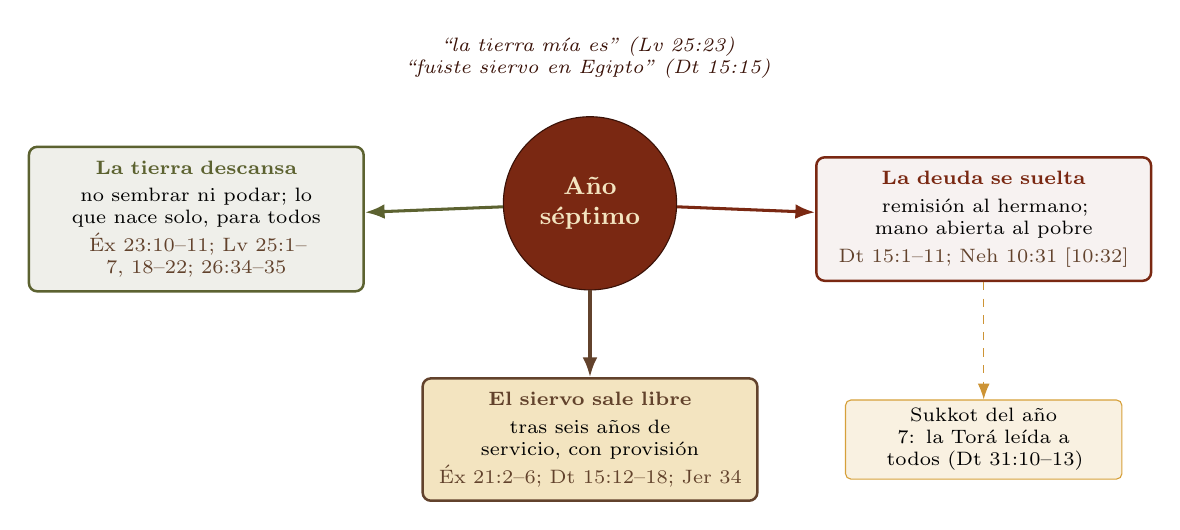
\begin{tikzpicture}[font=\scriptsize]
 \node[circle,fill=tierraroja,text=papiro,draw=caferojizo,minimum size=2.2cm,align=center,font=\small\bfseries] (c) at (0,0) {Año\\séptimo};
 \node[draw=oliva,line width=0.9pt,fill=oliva!10,rounded corners=3pt,text width=3.9cm,align=center,inner sep=5pt] (t) at (-5.0,-0.2) {\textbf{\color{oliva}La tierra descansa}\\[2pt] no sembrar ni podar; lo que nace solo, para todos\\[2pt]{\color{sepia}Éx 23:10--11; Lv 25:1--7, 18--22; 26:34--35}};
 \node[draw=sepia,line width=0.9pt,fill=papiro,rounded corners=3pt,text width=3.9cm,align=center,inner sep=5pt] (s) at (0,-3.0) {\textbf{\color{sepia}El siervo sale libre}\\[2pt] tras seis años de servicio, con provisión\\[2pt]{\color{sepia}Éx 21:2--6; Dt 15:12--18; Jer 34}};
 \node[draw=tierraroja,line width=0.9pt,fill=tierraroja!6,rounded corners=3pt,text width=3.9cm,align=center,inner sep=5pt] (d) at (5.0,-0.2) {\textbf{\color{tierraroja}La deuda se suelta}\\[2pt] remisión al hermano; mano abierta al pobre\\[2pt]{\color{sepia}Dt 15:1--11; Neh 10:31 [10:32]}};
 \draw[-{Latex[length=2.5mm]},line width=1.1pt,oliva] (c) -- (t);
 \draw[-{Latex[length=2.5mm]},line width=1.1pt,sepia] (c) -- (s);
 \draw[-{Latex[length=2.5mm]},line width=1.1pt,tierraroja] (c) -- (d);
 \node[text width=5.4cm,align=center,font=\scriptsize\itshape,text=caferojizo] at (0,1.85) {``la tierra mía es'' (Lv 25:23)\\ ``fuiste siervo en Egipto'' (Dt 15:15)};
 \node[draw=mostaza,fill=mostaza!15,rounded corners=2pt,text width=3.3cm,align=center,inner sep=3pt] (h) at (5.0,-3.0) {Sukkot del año 7: la Torá leída a todos (Dt 31:10--13)};
 \draw[-{Latex[length=2mm]},mostaza!90!tierraroja,dashed] (d) -- (h);
\end{tikzpicture}\par
{\footnotesize\color{sepia}\textit{Figura 5.} Los tres ámbitos del año séptimo y su fundamento. \textit{Nota.} Elaboración propia.}
\end{center}

%===================================================================
\section{Lectura histórica}

\subsection{Tierra, lluvia y deuda en el Israel agrario}
La tierra de Israel depende de la lluvia. La temprana del otoño ablanda el suelo para la siembra del trigo y la cebada; la tardía de la primavera llena la espiga (Dt 11:14; Jl 2:23). La cosecha de cereal va de Pésaj a Shavuot; la uva, el higo y la aceituna se recogen a fines del verano y en el otoño, antes de Sukkot. Un año de sequía, de langosta o de guerra deja a la familia sin semilla para el año siguiente, y a partir de ahí se pone en marcha el círculo que conocen todas las sociedades campesinas: la mala cosecha obliga a pedir prestado, el préstamo exige una prenda (Dt 24:6, 10--13) y, si no se paga, el acreedor toma la tierra o los hijos.

La Biblia muestra ese círculo en varios momentos. Una viuda clama a Eliseo: ``ha venido el acreedor para tomarse dos hijos míos por siervos'' (2~R 4:1). Amós acusa a Israel porque ``vendieron por dinero al justo, y al pobre por un par de zapatos'' (Am 2:6). En tiempos de Nehemías, el pueblo protesta porque ha empeñado sus tierras, viñas y casas para comprar grano, y algunos han entregado a sus hijas a servidumbre (Neh 5:1--5); Nehemías reprende a los nobles por los préstamos con interés (\heb{מַשָּׁא}, \emph{mashá}, Neh 5:7, 10) y los obliga a devolver campos y viñas (5:11--13). Las leyes de la shemitá responden a ese círculo impidiendo que la deuda se vuelva permanente y que la servidumbre sea hereditaria.

El descanso de la tierra tiene también un lado agrícola. El barbecho, dejar un campo sin sembrar para que recupere fuerza, era práctica conocida en la agricultura antigua, pero la ley bíblica no lo justifica por el rendimiento; lo funda en el sábado y en los pobres. Algunos autores han propuesto que Éx 23:10--11 pudo aplicarse al principio de modo rotativo, campo por campo, y que Lv 25 lo convirtió en un año único para todo el país (cf. de Vaux, 1985; Milgrom, 2001). Se trata de una hipótesis: el texto de Éxodo no lo dice, y el de Levítico supone un año común.

\subsection{El antiguo Cercano Oriente: edictos de \emph{mīšarum} y \emph{andurārum}}
Israel no fue el único pueblo antiguo que conoció la remisión de deudas. En Mesopotamia, los reyes de la época paleobabilónica proclamaban edictos de \emph{mīšarum} (``equidad, rectitud''), sobre todo al subir al trono y a veces durante el reinado. El más conocido es el de Ammi-saduqa de Babilonia (mediados del siglo \textsc{xvii} a.\,e.\,c., en la cronología media), que anula ciertas deudas de consumo de los súbditos de Akkad y Amurru, libera a quienes habían sido entregados por deudas y fija excepciones para los préstamos comerciales (Pritchard, 1969; Weinfeld, 1995). El término acadio para la liberación de personas es \emph{andurārum}, que la mayoría de los lexicógrafos relaciona con el hebreo \heb{דְּרוֹר} (\emph{derór}), la ``libertad'' de Lv 25:10 y Jer 34 (Koehler \& Baumgartner, 2001; Weinfeld, 1995).

El Código de Hammurabi (§117) limita la servidumbre por deudas de la esposa, el hijo o la hija a tres años; al cuarto quedan libres (Roth, 1997), en paralelo evidente con los seis años de Éx 21:2.

\begin{nota}[Precisión]
Los paralelos son reales, pero las diferencias pesan. (1) Los edictos mesopotámicos dependían de la voluntad del rey y eran irregulares; la shemitá es periódica y fija, y no depende del rey. (2) En Mesopotamia la remisión era un acto de gobierno; en Israel es un mandamiento de Dios dirigido a cada acreedor. (3) Ningún texto mesopotámico conocido da a la tierra un ``sábado''. Chirichigno (1993) y Weinfeld (1995) muestran que Israel comparte el vocabulario y la preocupación de su entorno, pero transforma la institución. No se puede afirmar una dependencia directa.
\end{nota}

\subsection{La shemitá en la historia narrada de Israel}
Los libros históricos no registran ninguna observancia del año séptimo antes del exilio; registran más bien su ausencia, pues Lv 26 y 2~Cr 36 suponen que Israel no lo guardó, y Jer 34 cuenta una liberación que duró poco. La única excepción posible es la señal dada a Ezequías durante la invasión asiria (701 a.\,e.\,c.):

\begin{cita}Y esto te daré por señal, oh Ezequías: Este año comeréis lo que nacerá de suyo, y el segundo año lo que nacerá de suyo; y el tercer año sembraréis, y segaréis, y plantaréis viñas, y comeréis el fruto de ellas.\fuente{(2~R 19:29; cf. Is 37:30)}\end{cita}

``Lo que nacerá de suyo'' es \heb{סָפִיחַ} (\emph{sefiaj}), la palabra de Lv 25:5. Dos años seguidos sin siembra recuerdan el año 49 y el año 50 del jubileo. Algunos cronólogos han propuesto que la señal coincidió con un año sabático seguido de un jubileo; otros piensan que la invasión simplemente impidió sembrar. Es una hipótesis que conviene marcar como tal; el vocabulario, sin embargo, une el relato con Lv 25.

Después del exilio, el pacto de Neh 10:31 [10:32] es el primer compromiso explícito con el año séptimo. Su fecha, a mediados del siglo \textsc{v} a.\,e.\,c., abre el período en que la práctica queda atestiguada.

\subsection{El Segundo Templo: una práctica atestiguada}
A partir de la época helenística, las fuentes muestran que la shemitá se guardaba y que tenía consecuencias políticas y militares.

\textbf{1 Macabeos.} Durante la campaña de Antíoco V y Lisias (163/162 a.\,e.\,c.), la fortaleza de Bet-sur se rinde por falta de víveres, porque era año sabático para la tierra (1~Mac 6:49). En Jerusalén, los defensores del templo tampoco tienen provisiones, por ser el año séptimo y porque los refugiados de entre los gentiles habían consumido las reservas (6:53). El año séptimo pesó en el resultado del asedio.

\textbf{Josefo.} El historiador judío registra varios datos. Según su relato, Alejandro Magno concedió a los judíos que en el año séptimo quedaran exentos de tributo (\emph{Ant.} 11.338). Juan Hircano levantó el asedio de una fortaleza cuando llegó el año en que los judíos descansan (\emph{Ant.} 13.234). Un decreto de Julio César exime a Judea del tributo en el año séptimo, porque en él no recogen fruto de los árboles ni siembran (\emph{Ant.} 14.202--206). Y el asedio de Jerusalén por Herodes (37 a.\,e.\,c.) coincidió con un año sabático, que agravó el hambre (\emph{Ant.} 14.475; 15.7).

\textbf{Tácito.} El historiador romano, hostil a los judíos, explica el sábado como pereza y añade que después, ``seducidos por la inercia'', dieron también a la ociosidad el séptimo año (\emph{Historias} 5.4, trad. propia). El texto es un prejuicio romano, pero confirma que a comienzos del siglo \textsc{ii} e.\,c. el año sabático se conocía fuera de Judea como rasgo de los judíos.

\textbf{Qumrán.} Los manuscritos del mar Muerto organizan el tiempo por ciclos sabáticos: el texto calendárico 4Q319 (\emph{Otot}) cuenta las señales por años de shemitá y jubileos (VanderKam, 1998). El manuscrito 11Q13 (11QMelquisedec) lee juntos Lv 25:13, Dt 15:2 e Is 61:1 y los aplica a los últimos días: Melquisedec proclamará la libertad en el décimo jubileo (García Martínez, 1992; Bergsma, 2007). Es el antecedente judío más claro de la lectura de Lc 4.

\textbf{Murabba'at.} Entre los papiros hallados en Wadi Murabba'at hay un pagaré arameo (Mur 18), fechado en el segundo año de Nerón (55/56 e.\,c.), que menciona el año de remisión (\heb{שְׁמִטָּה}) en su línea~7. Milik lo leyó como condicional: el deudor pagaría ``aunque sea año sabático'' (Benoit et al., 1961), lo que indicaría que los acreedores buscaban protegerse de la remisión; otros editores leen ``en este año de remisión'' y Wacholder (1973) prefiere esa lectura, que fecha el propio pagaré en un año sabático (otoño del 55 al del 56 e.\,c.). En ambos casos, el documento muestra que el cómputo de la shemitá seguía vigente en el siglo \textsc{i}.

\begin{nota}[Precisión]
Los datos de Josefo son de valor desigual: la concesión de Alejandro (\emph{Ant.} 11.338) pertenece a un relato legendario de su visita a Jerusalén; el decreto de César (\emph{Ant.} 14.202--206) es un documento que muchos historiadores consideran sustancialmente auténtico. La lectura condicional de Mur 18 es la de Milik en la edición de Benoit, Milik y de Vaux (1961) y está discutida; conviene citarla con prudencia. Las fechas exactas de los años sabáticos del Segundo Templo se reconstruyen con estos datos y difieren en un año según el sistema (Wacholder, 1973).
\end{nota}

\subsection{El exilio y los setenta años}
La cronología del exilio permite ver por qué los setenta años de Jeremías admiten varios cómputos. La figura muestra las fechas principales:

\begin{center}
\begin{tikzpicture}[font=\scriptsize,x=0.13cm]
 \draw[line width=1.4pt,tierraroja!80,-{Latex[length=3mm]}] (0,0) -- (112,0);
 \foreach \a/\x in {609/3,605/10,597/21,586/36,539/75,538/85,520/96,515/106}{
   \fill[mostaza] (\x,0) circle (3.2pt);
   \node[above=4pt,font=\scriptsize\bfseries,text=tierraroja] at (\x,0) {\a};}
 \foreach \x/\t/\r/\y in {3/{Muere Josías}/{2 R 23:29}/-0.3,10/{Carquemis; 1.ª deportación}/{Dn 1:1}/-1.35,21/{Joaquín deportado}/{2 R 24:12}/-0.3,36/{Templo destruido}/{2 R 25:8--9}/-1.35,75/{Cae Babilonia}/{Dn 5:30}/-0.3,85/{Edicto de Ciro}/{Esd 1:1}/-1.35,96/{``estos setenta años''}/{Zac 1:12}/-0.3,106/{Templo dedicado}/{Esd 6:15}/-1.35}{
   \draw[sepia!60] (\x,-0.12) -- (\x,\y);
   \node[below,text width=1.8cm,align=center,font=\tiny] at (\x,\y) {\textbf{\t}\\{\color{sepia}\r}};}
 \draw[decorate,decoration={brace,amplitude=5pt},oliva,line width=0.8pt] (10,0.85) -- (85,0.85) node[midway,above=6pt,font=\scriptsize,text=oliva] {605--538: unos 70 años de dominio babilonio y cautiverio};
 \draw[decorate,decoration={brace,amplitude=5pt},tierraroja,line width=0.8pt] (36,1.75) -- (106,1.75) node[midway,above=6pt,font=\scriptsize,text=tierraroja] {586--515: unos 70 años sin templo};
\end{tikzpicture}\par
{\footnotesize\color{sepia}\textit{Figura 6.} El exilio y los setenta años. \textit{Nota.} Elaboración propia. Fechas a.\,e.\,c., aproximadas; la destrucción del templo se fecha en 587 o 586 según el cómputo del año de Sedequías.}
\end{center}

Hay tres maneras principales de leer el número. (1) \emph{Desde el dominio babilonio}: de 605 (o 609) a la caída de Babilonia y el edicto de Ciro (539--538), unos setenta años; es la lectura que favorece Jer 25:11--12 (``servirán estas naciones al rey de Babilonia setenta años'') y Esd 1:1. (2) \emph{Desde la destrucción del templo}: de 586 a la dedicación del segundo templo (515), unos setenta años; es la perspectiva de Zac 1:12 y 7:5. (3) \emph{Como número redondo}: setenta años son ``los días de nuestra edad'' (Sal 90:10), una vida humana; una inscripción de Asarhadón de Asiria habla también de setenta años de abandono decretados para Babilonia. Las tres lecturas no se excluyen del todo, y el texto bíblico no fija el punto de partida.

\begin{nota}[Precisión: los 490 años]
2~Cr 36:21 relaciona los setenta años con los sábados de la tierra, pero no hace la aritmética. Una lectura tradicional, muy difundida en comentarios cristianos, razona así: si cada año sabático incumplido se ``cobró'' con un año de exilio, setenta años de exilio equivalen a setenta años sabáticos omitidos, es decir, $70\times 7 = 490$ años de desobediencia, aproximadamente la duración de la monarquía. Rashi (a Lv 26:35) hace otro cálculo: parte de los 390 años de pecado de Ez 4:5 (desde la entrada en la tierra hasta el exilio de las diez tribus), les suma los años de Judá (los 40 de Ez 4:6 más seis, hasta el exilio de Sedequías: 436 años) y cuenta en ellos los años sabáticos \emph{y} los jubileos incumplidos (dieciséis por cada siglo: catorce sabáticos y dos jubileos) hasta llegar a setenta. Ambos cálculos son interpretaciones; ninguno está en el texto bíblico. La relación con las ``setenta semanas'' de Dn 9:24 se trata en §6.4.
\end{nota}

%===================================================================
\section{Lectura filológica}

El vocabulario del año séptimo es concreto. Antes de ser términos técnicos, sus palabras describen gestos físicos: dejar caer, abandonar un campo, no cortar el pelo de la vid, abrir la mano. Los recuadros siguen el orden de los textos.

\begin{filologia}[\heb{שׁמט} \emph{shamat} y \heb{שְׁמִטָּה} \emph{shemitá}]
\begin{tabular}{@{}L{3.4cm}L{2.2cm}L{9.0cm}@{}}
\heb{כִּי שָׁמְטוּ הַבָּקָר} & 2~S 6:6 & ``porque los bueyes tropezaban'': el carro del arca se ladea y Uza la toca. El sentido físico es ``soltar, dejar caer, resbalar''. \\[2pt]
\heb{שִׁמְטֻהוּ} & 2~R 9:33 & ``Echadla abajo'': Jezabel es arrojada desde la ventana. \\[2pt]
\heb{נִשְׁמְטוּ} & Sal 141:6 & ``sean despeñados'' sus jueces. \\[2pt]
\heb{תִּשְׁמְטֶנָּה} & Éx 23:11 & ``la soltarás'' (la tierra): RVR1960 ``la dejarás libre''. \\[2pt]
\heb{שָׁמוֹט} & Dt 15:2 & infinitivo absoluto: ``soltar'' la deuda; RVR1960 ``perdonará''. \\[2pt]
\heb{שְׁמִטָּה} & Dt 15:1, 2, 9; 31:10 & sustantivo: ``suelta, remisión''. Solo en Deuteronomio (5 veces; conteo propio). \\
\end{tabular}\par\smallskip
La imagen es la de una mano que suelta lo que tenía agarrado: la tierra que se deja caer de la mano del dueño, la deuda que el acreedor deja de apretar. LXX traduce el verbo y el sustantivo con \grc{ἀφίημι} y \grc{ἄφεσις} (Éx 23:11; Dt 15:1--3).
\end{filologia}

\begin{filologia}[\heb{שַׁבָּת} \emph{shabat} y \heb{שַׁבָּתוֹן} \emph{shabatón}]
\begin{tabular}{@{}L{3.4cm}L{2.2cm}L{9.0cm}@{}}
\heb{וְשָׁבְתָה הָאָרֶץ} & Lv 25:2 & ``y la tierra descansará'': el verbo \emph{shavat}, ``cesar, detenerse'', con la tierra como sujeto. \\[2pt]
\heb{שַׁבַּת שַׁבָּתוֹן} & Lv 25:4 & ``sábado de reposo solemne'': superlativo hebreo (como ``cantar de los cantares''). El mismo título tienen el sábado semanal (Éx 31:15; Lv 23:3) y Yom Kipur (Lv 16:31; 23:32). \\[2pt]
\heb{שְׁנַת שַׁבָּתוֹן} & Lv 25:5 & ``año de reposo''. \emph{Shabatón} solo también designa Yom Teruá (Lv 23:24) y el primero y octavo día de Sukkot (23:39). \\[2pt]
\heb{שַׁבְּתֹתֶיהָ} & Lv 26:34, 43; 2~Cr 36:21 & ``sus sábados'': los años sabáticos de la tierra, que ella ``goza'' en el exilio. \\
\end{tabular}\par\smallskip
La palabra une el año séptimo con todo el reglamento de Lv 23. El vocabulario de las fiestas (\emph{shabatón}) y el del año séptimo es el mismo: la shemitá pertenece a la misma familia que las convocaciones santas.
\end{filologia}

\begin{filologia}[\heb{סָפִיחַ} \emph{sefiaj}]
\begin{tabular}{@{}L{3.4cm}L{2.2cm}L{9.0cm}@{}}
\heb{סְפִיחַ קְצִירְךָ} & Lv 25:5 & ``lo que de suyo naciere'' de tu siega: el grano caído que brota solo. \\[2pt]
\heb{אֶת־סְפִיחֶיהָ} & Lv 25:11 & lo mismo en el año del jubileo. \\[2pt]
\heb{סָפִיחַ} & 2~R 19:29; Is 37:30 & ``lo que nacerá de suyo'': la señal a Ezequías. \\
\end{tabular}\par\smallskip
El \emph{sefiaj} es lo que la tierra da sin trabajo humano. En el año séptimo, Israel come como en el Edén: de lo que Dios hace crecer, sin sembrar. La LXX lo traduce con \grc{τὰ αὐτόματα}, ``lo que brota por sí mismo'' (Lv 25:5, 11).
\end{filologia}

\begin{filologia}[\heb{נָזִיר} \emph{nazir}]
\begin{tabular}{@{}L{3.4cm}L{2.2cm}L{9.0cm}@{}}
\heb{עִנְּבֵי נְזִירֶךָ} & Lv 25:5, 11 & ``las uvas de tu \emph{nazir}'': la vid no podada. RVR1960 ``de tu viñedo''. \\[2pt]
\heb{נְזִיר אֱלֹהִים} & Jue 13:5; 16:17 & el nazareo, ``consagrado a Dios''. \\[2pt]
\heb{גַּדֵּל פֶּרַע} & Nm 6:5 & el nazareo deja crecer libremente el cabello, que no toca la navaja. \\
\end{tabular}\par\smallskip
La vid del año séptimo es una vid ``nazarea'': como el consagrado no se corta el cabello, la vid no se poda. La imagen es la de una tierra apartada para Dios por un año, consagrada como una persona (Milgrom, 2001; Hartley, 1992). Es un juego de palabras deliberado: el vocabulario del voto personal se aplica a la tierra.
\end{filologia}

\begin{filologia}[\heb{דְּרוֹר} \emph{derór}]
\begin{tabular}{@{}L{3.4cm}L{2.2cm}L{9.0cm}@{}}
\heb{וּקְרָאתֶם דְּרוֹר בָּאָרֶץ} & Lv 25:10 & ``pregonaréis libertad en la tierra'': el jubileo. \\[2pt]
\heb{לִקְרֹא לָהֶם דְּרוֹר} & Jer 34:8, 15, 17 & la libertad de Sedequías y la ``libertad a la espada''. \\[2pt]
\heb{לִקְרֹא לִשְׁבוּיִם דְּרוֹר} & Is 61:1 & ``a publicar libertad a los cautivos''. \\[2pt]
\heb{שְׁנַת הַדְּרוֹר} & Ez 46:17 & ``el año de la libertad'' (lit.; RVR1960: ``el año del jubileo''), cuando la heredad regalada vuelve al príncipe. \\[2pt]
\heb{דְּרוֹר} (ave) & Sal 84:3 [84:4] & ``la golondrina'' que halla nido: el ave que vuela libre. \\
\end{tabular}\par\smallskip
\emph{Derór} siempre se ``proclama'' (\emph{qará}): no es un sentimiento, sino un estatuto público. Se relaciona con el acadio \emph{andurārum} (§3.2). LXX lo traduce \grc{ἄφεσις} en Lv 25:10 e Is 61:1.
\end{filologia}

\begin{filologia}[\heb{אֶבְיוֹן} \emph{ebyón} y \heb{עָנִי} \emph{aní}]
\begin{tabular}{@{}L{3.4cm}L{2.2cm}L{9.0cm}@{}}
\heb{אֶבְיֹנֵי עַמֶּךָ} & Éx 23:11 & ``los pobres de tu pueblo'', que comen del campo en el año séptimo. \\[2pt]
\heb{לֹא יִהְיֶה־בְּךָ אֶבְיוֹן} & Dt 15:4 & ``que no haya en medio de ti mendigo'': el horizonte de la obediencia. \\[2pt]
\heb{לַעֲנִיֶּךָ וּלְאֶבְיֹנְךָ} & Dt 15:11 & ``al pobre y al menesteroso'': la pareja fija. \\
\end{tabular}\par\smallskip
\emph{Ebyón} es el que carece de lo necesario y depende de otro; \emph{aní} es el oprimido, el ``abajado''. En Dt 15 el sufijo posesivo es teológico: ``\emph{tu} pobre, \emph{tu} menesteroso'' (v.~11). El pobre no es un extraño, sino un pariente del que Israel responde. LXX traduce \emph{ebyón} de Dt 15:4 con \grc{ἐνδεής}, ``necesitado'' (§8.4).
\end{filologia}

\begin{filologia}[\heb{נָשָׁה} \emph{nashá}: prestar, ser acreedor]
\begin{tabular}{@{}L{3.4cm}L{2.2cm}L{9.0cm}@{}}
\heb{בַּעַל מַשֵּׁה יָדוֹ} & Dt 15:2 & ``el dueño del préstamo de su mano'': el acreedor (§5.1). \\[2pt]
\heb{אֲשֶׁר יַשֶּׁה בְּרֵעֵהוּ} & Dt 15:2 & ``que presta a su prójimo'' (hifil de \emph{nashá}). \\[2pt]
\heb{הַנֹּשֶׁה} & 2~R 4:1 & ``el acreedor'' que viene a llevarse a los hijos de la viuda. \\[2pt]
\heb{מַשָּׁא} & Neh 5:7, 10; 10:31 [10:32] & el préstamo con interés o la carga de la deuda. \\
\end{tabular}\par\smallskip
La raíz describe una relación de dependencia: el que presta ``tiene sobre'' el otro un derecho. El año séptimo corta ese derecho entre hermanos. La RVR1960 traduce la frase de Dt 15:2 con una paráfrasis: ``todo aquel que hizo empréstito de su mano, con el cual obligó a su prójimo''.
\end{filologia}

\subsection{La cadena más fuerte: de la shemitá al perdón}
La Septuaginta no tenía una palabra griega para cada matiz hebreo. Para la ``suelta'' de la tierra (Éx 23:11), la ``remisión'' de las deudas (Dt 15:1--3), la ``libertad'' del jubileo (Lv 25:10) y la ``libertad a los cautivos'' (Is 61:1) usó la misma familia: el verbo \grc{ἀφίημι}, ``soltar, dejar ir'', y el sustantivo \grc{ἄφεσις}, ``suelta, liberación''. Así, cuatro instituciones hebreas distintas llegaron al griego con una sola palabra.

\begin{center}\small\renewcommand{\arraystretch}{1.2}
\begin{tabular}{@{}L{2.2cm}L{3.8cm}L{4.4cm}L{4.0cm}@{}}
\toprule
\textbf{Texto} & \textbf{Hebreo (BHS)} & \textbf{LXX (Rahlfs-Hanhart)} & \textbf{Sentido} \\ \midrule
Éx 23:11 & \heb{תִּשְׁמְטֶנָּה} & \grc{ἄφεσιν ποιήσεις} & soltar la tierra \\
Dt 15:1 & \heb{תַּעֲשֶׂה שְׁמִטָּה} & \grc{ποιήσεις ἄφεσιν} & hacer remisión \\
Dt 15:2 & \heb{שָׁמוֹט} & \grc{ἀφήσεις πᾶν χρέος ἴδιον} & soltar toda deuda \\
Lv 25:10 & \heb{וּקְרָאתֶם דְּרוֹר} & \grc{διαβοήσετε ἄφεσιν} & pregonar libertad \\
Lv 25:10 & \heb{יוֹבֵל} & \grc{ἐνιαυτὸς ἀφέσεως σημασία} & el jubileo, ``año de la suelta'' \\
Is 61:1 & \heb{לִקְרֹא לִשְׁבוּיִם דְּרוֹר} & \grc{κηρύξαι αἰχμαλώτοις ἄφεσιν} & libertad a los cautivos \\
\bottomrule
\end{tabular}\par
{\footnotesize\color{sepia}\textit{Tabla 2.} \grc{ἄφεσις} en la Septuaginta. \textit{Nota.} Elaboración propia. La LXX de Jeremías (cap. 41 = TM 34) usa también \grc{ἄφεσις} para \emph{derór}: \grc{καλέσαι ἄφεσιν} (41:8, 15, 17).}
\end{center}

El Nuevo Testamento hereda la palabra con toda su carga. En Nazaret, Jesús lee Is 61:1 y añade una frase de Is 58:6, de modo que \grc{ἄφεσις} aparece dos veces: \grc{κηρύξαι αἰχμαλώτοις ἄφεσιν} y \grc{ἀποστεῖλαι τεθραυσμένους ἐν ἀφέσει} (Lc 4:18). En la oración que enseña a sus discípulos, la deuda y el perdón se dicen con el vocabulario de Dt 15:2 LXX: \grc{ἄφες ἡμῖν τὰ ὀφειλήματα ἡμῶν, ὡς καὶ ἡμεῖς ἀφήκαμεν τοῖς ὀφειλέταις ἡμῶν}, ``perdónanos nuestras deudas, como también nosotros perdonamos a nuestros deudores'' (Mt 6:12). Lucas da la versión con ``pecados'' y conserva la deuda en la segunda mitad: ``porque también nosotros perdonamos a todos los que nos deben'' (\grc{παντὶ ὀφείλοντι ἡμῖν}, Lc 11:4). En la última cena, la sangre del pacto es derramada \grc{εἰς ἄφεσιν ἁμαρτιῶν}, ``para remisión de los pecados'' (Mt 26:28), y Pedro anuncia el bautismo \grc{εἰς ἄφεσιν τῶν ἁμαρτιῶν} (Hch 2:38).

\begin{center}
\begin{tikzpicture}[font=\scriptsize,node distance=0.55cm]
 \node[draw=tierraroja,line width=0.8pt,fill=papiro,rounded corners=3pt,text width=3.25cm,align=center,inner sep=5pt] (h) {\textbf{Hebreo}\\[2pt] \heb{שְׁמִטָּה} \emph{shemitá}\\ (Éx 23:11; Dt 15:1--2)\\[2pt] \heb{דְּרוֹר} \emph{derór}\\ (Lv 25:10; Is 61:1)};
 \node[draw=tierraroja,line width=0.8pt,fill=papiro,rounded corners=3pt,text width=3.25cm,align=center,inner sep=5pt,right=of h] (l) {\textbf{Septuaginta}\\[2pt] \grc{ἄφεσις}, \grc{ἀφίημι}\\ ``suelta, soltar''\\[2pt] \grc{χρέος}, \grc{ὀφείλω}\\ ``deuda, deber''};
 \node[draw=mostaza,line width=1.5pt,fill=tierraroja,text=papiro,rounded corners=3pt,text width=3.25cm,align=center,inner sep=5pt,right=of l] (n) {\textbf{Nuevo Testamento}\\[2pt] \grc{ἄφεσιν} (Lc 4:18)\\ \grc{ἄφες\ldots\ ὀφειλήματα} (Mt 6:12)\\ \grc{εἰς ἄφεσιν ἁμαρτιῶν}\\ (Mt 26:28; Hch 2:38)};
 \node[draw=sepia,line width=0.8pt,fill=white,rounded corners=3pt,text width=2.6cm,align=center,inner sep=5pt,right=of n] (e) {\textbf{RVR1960}\\[2pt] ``remisión''\\ ``libertad''\\ ``perdónanos''\\ ``perdón''};
 \draw[-{Latex[length=3mm]},mostaza!90!tierraroja,line width=1.3pt] (h)--(l);
 \draw[-{Latex[length=3mm]},mostaza!90!tierraroja,line width=1.3pt] (l)--(n);
 \draw[-{Latex[length=3mm]},mostaza!90!tierraroja,line width=1.3pt] (n)--(e);
 \node[below=0.35cm of l,text width=12cm,align=center,font=\scriptsize\itshape,text=sepia,xshift=1.8cm] {la tierra soltada, la deuda remitida y el cautivo liberado se dicen en griego con la misma palabra que el perdón de los pecados};
\end{tikzpicture}\par
{\footnotesize\color{sepia}\textit{Figura 7.} De la shemitá al perdón: hebreo $\rightarrow$ LXX $\rightarrow$ NT $\rightarrow$ español. \textit{Nota.} Elaboración propia con la BHS, Rahlfs-Hanhart y NA28.}
\end{center}

La cadena es filológica antes que teológica: muestra cómo un lector judío de habla griega del siglo \textsc{i} oía la palabra \grc{ἄφεσις}. Cuando un evangelio decía ``remisión de pecados'', ese lector tenía en el oído la remisión de las deudas, la tierra soltada y la libertad del jubileo. La oración del Señor hace explícita la relación: el pecado es una deuda (\grc{ὀφείλημα}), y el perdón es su remisión. Jesús lo desarrolla en la parábola del siervo a quien el rey ``le perdonó la deuda'' (\grc{τὸ δάνειον ἀφῆκεν αὐτῷ}, Mt 18:27) y que después no quiso soltar a su consiervo (18:23--35): un Dt 15 en forma de relato.

\begin{nota}[Precisión]
En el griego del NT, \grc{ἄφεσις} significa ante todo ``perdón'' (BDAG). Que en cada uso resuene la shemitá es una conclusión de lectura, más fuerte en Lc 4:18 (cita de Is 61 y 58) y en Mt 6:12 y 18:23--35 (vocabulario de deuda) que en Hch 2:38. La cadena léxica es segura; la intención de cada autor se discute (Sloan, 1977; Bergsma, 2007).
\end{nota}

%===================================================================
\section{Lectura textual}

\subsection{Dt 15:2: una sintaxis difícil}
La primera frase de la ley de remisión es una de las más discutidas de Deuteronomio:

\hebverso{שָׁמוֹט כָּל־בַּעַל מַשֵּׁה יָדוֹ אֲשֶׁר יַשֶּׁה בְּרֵעֵהוּ}

Una traducción literal sería: ``soltar [ha de soltar] todo dueño de préstamo de su mano lo que preste a su prójimo''. El problema es qué funciona como sujeto y qué como objeto. Hay dos lecturas principales. (a) \emph{Kol báal mashé yadó} es el sujeto (``todo acreedor'') y la oración de relativo \emph{asher yashé bereehu} es el objeto (``lo que haya prestado a su prójimo''): ``todo acreedor soltará lo que prestó a su prójimo''. Es la lectura de la mayoría de las versiones modernas y de Tigay (1996). (b) \emph{Báal} se toma en sentido técnico y \emph{mashé yadó} como ``la prenda de su mano'': lo que se suelta sería la prenda o el derecho de cobro, no necesariamente la deuda entera. Esta segunda lectura alimenta un debate antiguo: ¿la shemitá cancela la deuda o solo suspende su cobro durante el año? La tradición rabínica entiende cancelación (Misná \emph{Sheviít} 10:1); algunos intérpretes medievales y modernos hablan de suspensión. El v.~2b (``no lo demandará más'') y la preocupación de v.~9 favorecen la cancelación: si solo se suspendiera el cobro, el acreedor no tendría motivo para negarse a prestar (Hamilton, 1992).

La LXX resuelve la sintaxis a su modo: \grc{ἀφήσεις πᾶν χρέος ἴδιον, ὃ ὀφείλει σοι ὁ πλησίον}, ``soltarás toda deuda propia que te deba el prójimo''. Convierte la ley en segunda persona y pone el acento en la deuda.

\subsection{Lv 25:5--6: ¿se puede comer lo que nace solo?}
El v.~5 prohíbe segar el \emph{sefiaj} y vendimiar la vid no podada; el v.~6 dice que ``el descanso de la tierra te dará de comer''. ¿Se puede comer o no? La tensión se resuelve con los verbos: lo prohibido es \heb{תִקְצוֹר} (\emph{tiqtsor}, ``segar'') y \heb{תִבְצֹר} (\emph{tivtsor}, ``vendimiar''), es decir, la cosecha organizada y almacenada del dueño. Lo permitido es comer de lo que el campo da, sin almacenarlo como propiedad. Milgrom (2001) entiende que el dueño puede tomar para su consumo inmediato, igual que el pobre y el extranjero, pero no puede cosechar como en los otros años. La tradición rabínica lo formula como \emph{hefqer}: en el año séptimo el fruto es ``sin dueño'' y cualquiera puede tomarlo (tratado \emph{Sheviít} de la Misná, tradición posterior).

\subsection{2~Cr 36:21: una cita compuesta}
El cronista dice que todo ocurrió ``para que se cumpliese la palabra de \SENOR{} por boca de Jeremías'', pero la frase siguiente, ``hasta que la tierra hubo gozado de reposo'', no está en Jeremías: viene de Lv 26:34--35. El cronista funde dos textos y atribuye el conjunto al profeta. Es una práctica conocida de citación libre en la Biblia hebrea y en el NT (cf. Mr 1:2--3, que en el texto crítico reúne Mal 3:1 e Is 40:3 bajo ``Isaías''; la RVR1960 lee ``en los profetas''). La fusión es interpretativa: el cronista entiende los setenta años de Jeremías como el tiempo en que se cumple la amenaza de Levítico.

\subsection{Dt 15:18: ``la mitad'' o ``el doble''}
La RVR1960 traduce: ``por la mitad del costo de un jornalero te sirvió seis años''. El hebreo dice \heb{מִשְׁנֶה שְׂכַר שָׂכִיר} (\emph{mishné sejar sajir}). \emph{Mishné} significa normalmente ``doble'' o ``segundo'' (Gn 43:12; Is 61:7). La frase puede leerse como ``el doble del salario de un jornalero'' (el siervo trabajó día y noche, o sin salario, y le costó al amo la mitad de lo que habría pagado a un asalariado) o como ``el equivalente'' del salario (Tigay, 1996). La RVR1960 traduce el sentido económico (al amo le costó la mitad), no la palabra.

\begin{nota}[Precisión textual]
(1) \emph{Al cabo de siete años}: la expresión \heb{מִקֵּץ שֶׁבַע שָׁנִים} (Dt 15:1; 31:10; Jer 34:14) no significa ``después de siete años completos'', sino ``al llegar el séptimo''. Jer 34:14 lo muestra al añadir ``le servirá seis años''. (2) En Lv 26:34 el TM lee \heb{הֳשַׁמָּה} y en 26:35 \heb{הָשַּׁמָּה}; son dos vocalizaciones de la misma forma verbal (``estar desolada''). (3) La LXX de Dt 15:2 convierte la ley en segunda persona (\grc{ἀφήσεις}); la traducción española sigue el TM. (4) En Lv 25:5 la RVR1960 traduce \emph{nezireja} por ``tu viñedo'' y pierde el juego con el nazareato (§4).
\end{nota}

\subsection{El cómputo de la cosecha triple}
Lv 25:21--22 promete fruto ``por tres años'' y dice que se sembrará el año octavo y se comerá del añejo ``hasta el año noveno''. Si el año comienza en primavera (Nisán), la cosecha del sexto alcanza para el séptimo y el octavo, y la del octavo llega en su primavera. Si el año agrícola comienza en otoño (Tishri), como supone Lv 25:9 para el jubileo, el cómputo cambia: la siembra del octavo se hace en su otoño y la cosecha llega en la primavera del noveno. Los comentarios discuten además cómo encaja la promesa cuando el año 49 (sabático) y el año 50 (jubileo) caen seguidos (Milgrom, 2001; Bergsma, 2007). La cuestión se estudia en el capítulo 09.

%===================================================================
\section{Lectura literaria}

\subsection{La escalera del siete}
La Torá organiza el tiempo sagrado con el número siete en escala creciente. Cada escalón multiplica o prolonga el anterior: el séptimo día (Gn 2:2--3; Éx 20:8--11; Lv 23:3); las siete semanas del ómer, que terminan en Shavuot, el día cincuenta (Lv 23:15--16); el mes séptimo, que concentra Yom Teruá, Yom Kipur y Sukkot (Lv 23:23--43); el año séptimo, la shemitá (Lv 25:1--7); y las siete semanas de años, que terminan en el año cincuenta, el jubileo (Lv 25:8--12). Las dos series paralelas, la de los días y la de los años, terminan en un ``cincuenta'': Shavuot y el \emph{yovel}.

\begin{center}
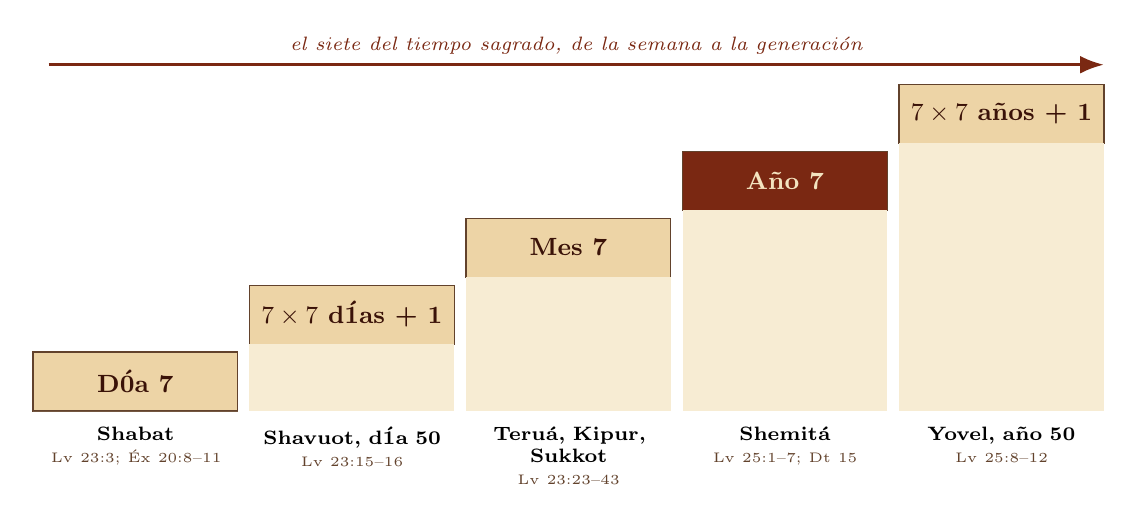
\begin{tikzpicture}[font=\scriptsize,x=1cm,y=1cm]
 \foreach \i/\t/\d/\r in {0/{Día 7}/{Shabat}/{Lv 23:3; Éx 20:8--11},1/{$7\times7$ días + 1}/{Shavuot, día 50}/{Lv 23:15--16},2/{Mes 7}/{Teruá, Kipur, Sukkot}/{Lv 23:23--43},3/{Año 7}/{Shemitá}/{Lv 25:1--7; Dt 15},4/{$7\times7$ años + 1}/{Yovel, año 50}/{Lv 25:8--12}}{
   \pgfmathsetmacro{\x}{\i*2.75}
   \pgfmathsetmacro{\y}{\i*0.85}
   \ifnum\i=3
     \fill[tierraroja] (\x,\y) rectangle ++(2.6,0.75);
     \node[text=papiro,font=\small\bfseries] at (\x+1.3,\y+0.38) {\t};
   \else
     \fill[mostaza!45] (\x,\y) rectangle ++(2.6,0.75);
     \node[text=caferojizo,font=\small\bfseries] at (\x+1.3,\y+0.38) {\t};
   \fi
   \draw[sepia,line width=0.5pt] (\x,\y) rectangle ++(2.6,0.75);
   \fill[papiro!70] (\x,0) rectangle ++(2.6,\y);
   \node[anchor=north,text width=2.5cm,align=center,font=\scriptsize] at (\x+1.3,-0.08) {\textbf{\d}\\{\color{sepia}\tiny \r}};}
 \draw[-{Latex[length=3mm]},tierraroja,line width=1pt] (0.2,4.4) -- (13.6,4.4) node[midway,above,font=\scriptsize\itshape,text=tierraroja] {el siete del tiempo sagrado, de la semana a la generación};
\end{tikzpicture}\par
{\footnotesize\color{sepia}\textit{Figura 8.} La escalera del siete. \textit{Nota.} Elaboración propia con Lv 23 y Lv 25. El escalón resaltado es el de este estudio.}
\end{center}

La escalera muestra una lógica de extensión. El sábado semanal libera al trabajador y al animal por un día; el año séptimo libera a la tierra, al siervo y al deudor por un año; el jubileo devuelve la tierra a la familia y al israelita a su clan. Cada escalón amplía el alcance del reposo. La shemitá ocupa el lugar central: es el primer escalón que mide el tiempo en años y el que da su unidad al jubileo (``siete semanas de años'', Lv 25:8).

\subsection{El ciclo de cuarenta y nueve años}
Lv 25:8 manda contar \heb{שֶׁבַע שַׁבְּתֹת שָׁנִים} (\emph{shéva shabtot shanim}), ``siete sábados de años'', ``siete veces siete años''. La palabra para ``semana de años'' es \emph{shabat}: cada heptada se cierra con su sábado. La cuadrícula siguiente muestra el ciclo completo:

\begin{center}
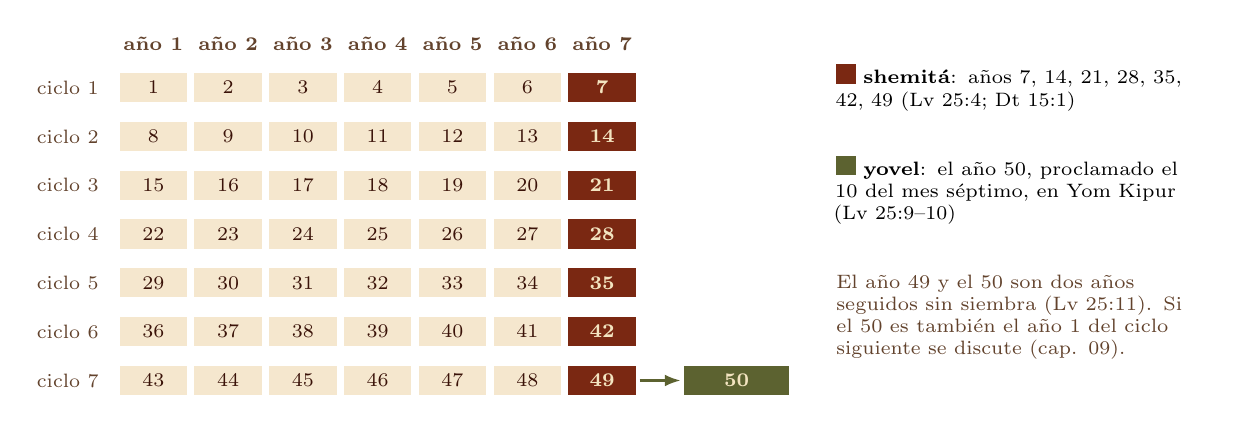
\begin{tikzpicture}[font=\scriptsize,x=0.95cm,y=0.62cm]
 \foreach \c in {1,...,7}{\node[font=\scriptsize\bfseries,text=sepia] at (\c,0.9) {año \c};}
 \foreach \r in {1,...,7}{
   \node[font=\scriptsize,text=sepia,anchor=east] at (0.4,-\r+1) {ciclo \r};
   \foreach \c in {1,...,7}{
     \pgfmathtruncatemacro{\n}{(\r-1)*7+\c}
     \ifnum\c=7
       \fill[tierraroja] (\c-0.45,-\r+0.7) rectangle (\c+0.45,-\r+1.3);
       \node[text=papiro,font=\scriptsize\bfseries] at (\c,-\r+1) {\n};
     \else
       \fill[mostaza!25] (\c-0.45,-\r+0.7) rectangle (\c+0.45,-\r+1.3);
       \node[text=caferojizo] at (\c,-\r+1) {\n};
     \fi}}
 \fill[oliva] (8.1,-6.3) rectangle (9.5,-5.7);
 \node[text=papiro,font=\scriptsize\bfseries] at (8.8,-6.0) {50};
 \draw[-{Latex[length=2mm]},oliva,line width=0.9pt] (7.5,-6.0) -- (8.05,-6.0);
 \node[anchor=west,text width=4.6cm,font=\scriptsize] at (10.0,0.0) {\textcolor{tierraroja}{\rule{2.5mm}{2.5mm}} \textbf{shemitá}: años 7, 14, 21, 28, 35, 42, 49 (Lv 25:4; Dt 15:1)};
 \node[anchor=west,text width=4.6cm,font=\scriptsize] at (10.0,-2.1) {\textcolor{oliva}{\rule{2.5mm}{2.5mm}} \textbf{yovel}: el año 50, proclamado el 10 del mes séptimo, en Yom Kipur (Lv 25:9--10)};
 \node[anchor=west,text width=4.6cm,font=\scriptsize,text=sepia] at (10.0,-4.7) {El año 49 y el 50 son dos años seguidos sin siembra (Lv 25:11). Si el 50 es también el año 1 del ciclo siguiente se discute (cap. 09).};
\end{tikzpicture}\par
{\footnotesize\color{sepia}\textit{Figura 9.} El ciclo de cuarenta y nueve años con los siete años sabáticos y el jubileo. \textit{Nota.} Elaboración propia con Lv 25:1--12.}
\end{center}

\subsection{Lv 25--26 como unidad}
Los capítulos 25 y 26 de Levítico forman un bloque enmarcado por el Sinaí. Lv 25:1 abre: ``\SENOR{} habló a Moisés en el monte de Sinaí''; Lv 26:46 cierra: ``Estos son los estatutos, ordenanzas y leyes que estableció \SENOR{} entre sí y los hijos de Israel en el monte de Sinaí por mano de Moisés''. Es una inclusión.

La presentación de Danilo sobre el jubileo propone una síntesis de Lv 25 que muestra la lógica interna del capítulo: (1) el año sabático (vv.~1--7); (2) el año del jubileo (vv.~8--17), con dos desarrollos: (2.1) la consecuencia de la obediencia (vv.~18--22: la tierra dará su fruto y ``habitaréis en ella con seguridad''), y (2.2) las consecuencias de la santidad, que se despliegan en dos planos: \emph{de la tierra}, el rescate de las propiedades (vv.~23--34: ``la tierra mía es'', v.~23; el pariente más cercano rescata, v.~25), y \emph{del pueblo}, el préstamo y la manumisión (vv.~35--55). El cierre lo da Lv 26:2: ``Guardad mis días de reposo, y tened en reverencia mi santuario''. Sus notas añaden los detalles que muestran el espíritu del capítulo: obrar con temor de Dios y no explotarse en las transacciones (25:14--17); las casas en ciudades amuralladas tienen un año de plazo de rescate y no vuelven en el jubileo, salvo las de los levitas (25:29--34); al hermano empobrecido se le presta sin interés y, si se vende, sirve como jornalero y no como esclavo hasta el jubileo (25:35--43); si se vende a un extranjero, un familiar lo rescata o sale en el jubileo (25:47--55).

\begin{center}
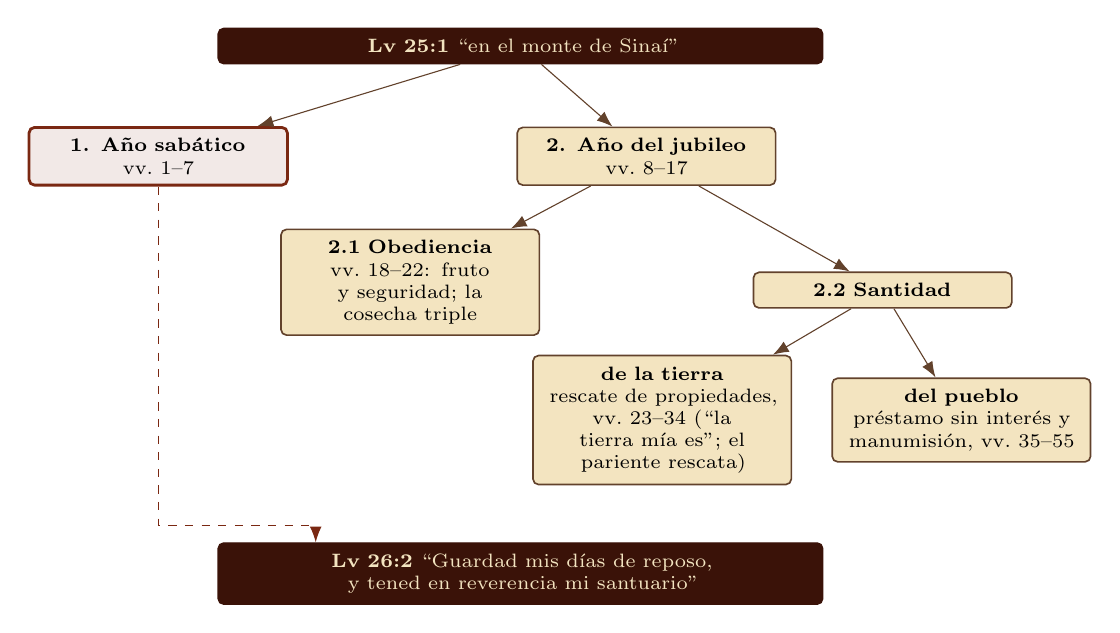
\begin{tikzpicture}[font=\scriptsize,
  bl/.style={draw=sepia,line width=0.6pt,fill=papiro,rounded corners=2pt,text width=3.0cm,align=center,inner sep=4pt},
  rj/.style={draw=tierraroja,line width=1pt,fill=tierraroja!10,rounded corners=2pt,text width=3.0cm,align=center,inner sep=4pt}]
 \node[draw=caferojizo,fill=caferojizo,text=papiro,rounded corners=2pt,text width=7.4cm,align=center,inner sep=4pt] (s) at (0,0) {\textbf{Lv 25:1} ``en el monte de Sinaí''};
 \node[rj] (a) at (-4.6,-1.4) {\textbf{1. Año sabático}\\ vv.~1--7};
 \node[bl] (b) at (1.6,-1.4) {\textbf{2. Año del jubileo}\\ vv.~8--17};
 \node[bl] (b1) at (-1.4,-3.0) {\textbf{2.1 Obediencia}\\ vv.~18--22: fruto y seguridad; la cosecha triple};
 \node[bl] (b2) at (4.6,-3.1) {\textbf{2.2 Santidad}};
 \node[bl] (t) at (1.8,-4.75) {\textbf{de la tierra}\\ rescate de propiedades, vv.~23--34 (``la tierra mía es''; el pariente rescata)};
 \node[bl] (p) at (5.6,-4.75) {\textbf{del pueblo}\\ préstamo sin interés y manumisión, vv.~35--55};
 \node[draw=caferojizo,fill=caferojizo,text=papiro,rounded corners=2pt,text width=7.4cm,align=center,inner sep=4pt] (c) at (0,-6.7) {\textbf{Lv 26:2} ``Guardad mis días de reposo, y tened en reverencia mi santuario''};
 \draw[-{Latex[length=2mm]},sepia] (s) -- (a); \draw[-{Latex[length=2mm]},sepia] (s) -- (b);
 \draw[-{Latex[length=2mm]},sepia] (b) -- (b1); \draw[-{Latex[length=2mm]},sepia] (b) -- (b2);
 \draw[-{Latex[length=2mm]},sepia] (b2) -- (t); \draw[-{Latex[length=2mm]},sepia] (b2) -- (p);
 \draw[-{Latex[length=2mm]},tierraroja,dashed] (a.south) -- ++(0,-4.3) -| ([xshift=-2.6cm]c.north);
\end{tikzpicture}\par
{\footnotesize\color{sepia}\textit{Figura 10.} Lv 25 según la síntesis de Danilo, con su cierre en Lv 26:2. \textit{Nota.} Elaboración propia a partir de la presentación \emph{El Jubileo} del autor de la serie.}
\end{center}

Lv 26 continúa el bloque: bendiciones (26:3--13), en que la tierra da su fruto (26:4; cf. 25:19); maldiciones (26:14--39), en que la tierra ``goza sus sábados'' (26:34--35); y confesión con memoria del pacto: ``me acordaré de la tierra'' (26:40--45). La lectura de López (1994) coincide en el núcleo: el año sabático es una institución cultual ``cuyo sentido fundamental es la justicia y la solidaridad'', y Lv 25 la desarrolla en dos acciones, el rescate de la tierra perdida por deudas y el rescate de las personas sometidas por deudas.

Tres rasgos dan unidad al bloque. Primero, el sábado: el bloque comienza con el sábado de la tierra (25:2) y la bisagra entre leyes y sanciones repite ``guardad mis días de reposo'' (26:2). Segundo, el número siete: las maldiciones se intensifican ``siete veces'' (26:18, 21, 24, 28), cuatro veces la misma fórmula. El pueblo que no respeta el ritmo de siete en el tiempo recibe el castigo multiplicado por siete. Tercero, la tierra como actor: en Lv 25 ``guarda sábado''; en Lv 26 da o niega su fruto, ``goza'' sus sábados y es ``recordada'' por Dios (26:42). La bendición y la maldición están ligadas a la tierra porque la tierra es de Dios.

El estribillo de Lv 25:38, 42 y 55 explica por qué el israelita no puede ser esclavo de otro israelita: ``porque son mis siervos, los cuales saqué yo de la tierra de Egipto'' (25:42). Los siervos del \SENOR{} no pueden ser vendidos ``a manera de esclavos''. La teología del éxodo y la de la shemitá se apoyan mutuamente: la tierra es de Dios y el pueblo es de Dios.

\subsection{Daniel 9: setenta semanas de años}
Daniel lee a Jeremías durante el primer año de Darío: ``yo Daniel miré atentamente en los libros el número de los años de que habló \SENOR{} al profeta Jeremías, que habían de cumplirse las desolaciones de Jerusalén en setenta años'' (Dn 9:2). Después de su oración, Gabriel le responde con una multiplicación:

\hebverso{שָׁבֻעִים שִׁבְעִים נֶחְתַּךְ עַל־עַמְּךָ וְעַל־עִיר קָדְשֶׁךָ}
\begin{cita}Setenta semanas están determinadas sobre tu pueblo y sobre tu santa ciudad, para terminar la prevaricación, y poner fin al pecado, y expiar la iniquidad, para traer la justicia perdurable, y sellar la visión y la profecía, y ungir al Santo de los santos.\fuente{(Dn 9:24)}\end{cita}

\emph{Shavuim shivim}, ``setenta semanas'', son setenta heptadas. La mayoría de los intérpretes, antiguos y modernos, las entiende como heptadas de años: $70\times 7 = 490$ años. La relación con Lv 25--26 es estrecha: los setenta años de Jeremías se multiplican por siete, como las maldiciones de Lv 26 (``siete veces más''), y 490 años equivalen a diez jubileos ($10\times 49$). Daniel reinterpreta el exilio con la aritmética del año sabático. Se ha propuesto que Dn 9 entiende el fin del exilio verdadero como un gran jubileo (Bergsma, 2007), en línea con 11Q13, que habla del ``décimo jubileo'' (§3.4).

\begin{center}
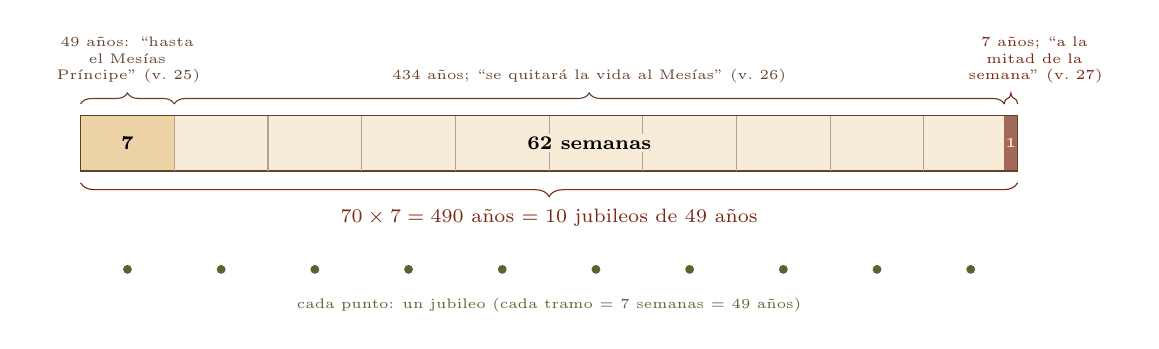
\begin{tikzpicture}[font=\scriptsize,x=0.17cm]
 \fill[mostaza!45] (0,0) rectangle (7,0.7);
 \fill[mostaza!20] (7,0) rectangle (69,0.7);
 \fill[tierraroja!70] (69,0) rectangle (70,0.7);
 \draw[sepia] (0,0) rectangle (70,0.7);
 \foreach \x in {7,14,...,63}{\draw[sepia!50] (\x,0) -- (\x,0.7);}
 \node[font=\scriptsize\bfseries] at (3.5,0.35) {7};
 \node[font=\scriptsize\bfseries,fill=mostaza!20,inner sep=1pt] at (38,0.35) {62 semanas};
 \node[font=\tiny\bfseries,text=papiro] at (69.5,0.35) {1};
 \draw[decorate,decoration={brace,amplitude=4pt},sepia] (0,0.85) -- (7,0.85) node[midway,above=4pt,text width=2.3cm,align=center,font=\tiny] {49 años: ``hasta el Mesías Príncipe'' (v.~25)};
 \draw[decorate,decoration={brace,amplitude=4pt},sepia] (7,0.85) -- (69,0.85) node[midway,above=4pt,font=\tiny] {434 años; ``se quitará la vida al Mesías'' (v.~26)};
 \draw[decorate,decoration={brace,amplitude=4pt},tierraroja] (69,0.85) -- (70,0.85) node[midway,above=4pt,text width=2.2cm,align=center,font=\tiny,text=tierraroja,xshift=0.3cm] {7 años; ``a la mitad de la semana'' (v.~27)};
 \draw[decorate,decoration={brace,amplitude=5pt,mirror},tierraroja] (0,-0.15) -- (70,-0.15) node[midway,below=6pt,font=\scriptsize,text=tierraroja] {$70\times 7 = 490$ años $= 10$ jubileos de 49 años};
 \foreach \j in {1,...,10}{\pgfmathsetmacro{\xj}{\j*7-3.5}\fill[oliva] (\xj,-1.25) circle (1.6pt);}
 \node[font=\tiny,text=oliva] at (35,-1.7) {cada punto: un jubileo (cada tramo = 7 semanas = 49 años)};
\end{tikzpicture}\par
{\footnotesize\color{sepia}\textit{Figura 11.} Las setenta semanas de Dn 9:24--27 como heptadas de años. \textit{Nota.} Elaboración propia. Esquema \emph{interpretativo}: la división $7 + 62 + 1$ está en el texto; los puntos de partida y de llegada se discuten.}
\end{center}

\begin{nota}[Precisión: lecturas de Dn 9]
Que las ``semanas'' sean de años es la lectura mayoritaria, pero el texto no lo dice. Las lecturas principales son: (1) \emph{mesiánica}: desde un decreto persa (Ciro, 538; Artajerjes, 457 o 444 a.\,e.\,c.) hasta el ministerio y la muerte de Jesús; la defienden comentaristas conservadores y la tradición adventista; (2) \emph{macabea}: desde el exilio o la palabra de Jeremías hasta la profanación del templo por Antíoco IV (167--164 a.\,e.\,c.); es la lectura de la mayoría de los críticos (Collins, 1993); (3) \emph{dispensacionalista}: 69 semanas hasta Cristo y una semana final separada, futura. Todos los cálculos son interpretativos. Este capítulo se limita a mostrar que Dn 9 piensa con los ciclos sabáticos; el jubileo se estudia en el capítulo 09.
\end{nota}

\subsection{Intertextualidad: la tierra, el maná y el Edén}
Tres textos anteriores iluminan el año séptimo. El \emph{maná} (Éx 16) enseña la misma pedagogía: el sexto día cae doble, el séptimo no cae, y el que sale a recoger ``no halló'' (16:27). Lv 25:20--22 aplica la misma lección a los años. La \emph{creación} (Gn 1--2) ofrece el modelo: Dios trabaja seis días y en el séptimo ``reposó'' (\heb{וַיִּשְׁבֹּת}, Gn 2:2); la tierra de Lv 25 imita a su Creador. El \emph{Edén} ofrece la imagen: el hombre fue puesto en el huerto ``para que lo labrara y lo guardase'' (Gn 2:15), y comía de lo que Dios hacía brotar (2:9). En el año séptimo, Israel vuelve por un año a esa condición: come lo que nace solo, sin poseerlo. La lectura es intertextual y conviene marcarla como tal, pero el vocabulario del reposo (\emph{shavat}) une los tres textos.

%===================================================================
\section{Memorial, figura y esperanza: la lectura de la serie}

El documento de referencia de la serie (lecciones 6--14 de un curso de doctrina de la adoración, en la línea de la Iglesia de Dios) no dedica una lección al año sabático. Pero su marco permite situarlo con precisión. Esta sección expone ese marco y lo aplica a la shemitá; las precisiones se marcan.

\subsection{El reglamento del culto y el sábado}
Para la serie, Lv 23 es el \emph{reglamento del culto}: las ``solemnidades de \SENOR'' (\emph{moadé YHWH}) que Israel debe proclamar como ``santas convocaciones'', es decir, ``citaciones santas'' ordenadas por Dios, ``en sus tiempos'' y como ``estatuto perpetuo''. El documento distingue ese reglamento de la ``ley de los sacrificios'' (Lv 1--7; Nm 28--29), que proveía la remisión del pecado mediante la sangre y que Pablo llama ``la ley de los mandamientos expresados en ordenanzas''. El primer renglón del reglamento es el sábado (Lv 23:3), que el documento presenta como mandato instituido por Dios, memorial de la creación, señal entre Dios y su pueblo, estatuto perpetuo y ``símbolo de la vida eterna después del Milenio''.

La shemitá pertenece a ese primer renglón. No es una convocación anual ni requiere sacrificios propios: es el sábado proyectado sobre los años. Su título es el del sábado (\emph{shabat shabatón}, \emph{shabat laYHWH}), y su lugar en la Torá es el Sinaí (Lv 25:1), como el reglamento del culto.

\subsection{Memorial: ``te acordarás de que fuiste siervo''}
En la serie, cada fiesta es memorial de un hito de la historia de Israel. La shemitá tiene su memorial explícito en el texto: ``Y te acordarás de que fuiste siervo en la tierra de Egipto, y que \SENOR{} tu Dios te rescató'' (Dt 15:15). Lv 25 lo repite en su estribillo: ``Yo \SENOR{} vuestro Dios, que os saqué de la tierra de Egipto'' (25:38; cf. 25:55). El año séptimo hace memoria de la salida de Egipto, el hito de Pésaj y de Matsot, y la extiende a la economía: el pueblo que fue liberado no puede esclavizar a su hermano.

El texto añade una cláusula que la serie puede leer como hito propio: ``Cuando hayáis entrado en la tierra que yo os doy, la tierra guardará reposo'' (Lv 25:2). La shemitá supone la entrada en Canaán, el hito que la serie asocia con Josué. Y aquí aparece su punto más fuerte: el sábado de la tierra comenzó con la entrada y terminó, por incumplimiento, con el exilio (Lv 26:34--35; 2~Cr 36:21). Israel entró en la tierra, pero no ``reposó'' en ella como Dios quería.

\subsection{Figura: el reposo que no se alcanzó con Josué}
Para la serie, el sábado representa en el plan de salvación el reposo del que dice Hebreos: ``queda un reposo para el pueblo de Dios'' (He 4:9), no alcanzado con Josué, y que se cumple en el encuentro de Dios con sus hijos en la Jerusalén celestial (Ap 21:1--4). El documento cita Hebreos:

\begin{cita}Porque si Josué les hubiera dado el reposo, no hablaría después de otro día. Por tanto, queda un reposo para el pueblo de Dios. Porque el que ha entrado en su reposo, también ha reposado de sus obras, como Dios de las suyas.\fuente{(He 4:8--10)}\end{cita}

``Reposo'' en He 4:9 es \grc{σαββατισμός}, ``guarda de sábado'', una palabra rara, que no aparece en la Septuaginta. La historia de la shemitá ilustra el argumento de Hebreos con precisión: la tierra que Josué dio a Israel tuvo sábados prescritos que Israel no guardó; la tierra los ``cobró'' en el exilio; el reposo verdadero quedó pendiente. Lo que la serie dice del sábado semanal se puede decir, con más fuerza todavía, del sábado de la tierra.

\begin{center}\small\renewcommand{\arraystretch}{1.22}
\begin{tabular}{@{}L{4.1cm}L{4.6cm}L{5.6cm}@{}}
\toprule
\textbf{Hito de Israel} & \textbf{Shemitá} & \textbf{Nuevo Pacto (lectura de la serie)} \\ \midrule
Salida de Egipto: ``fuiste siervo'' (Dt 15:15) & el siervo sale libre y con provisión & libertad del pecado y de su servidumbre (Jn 8:34--36; Ro 6:22--23) \\
Entrada en la tierra con Josué (Lv 25:2) & la tierra guarda sábado para el \SENOR{} & el reposo que queda (He 4:8--9) \\
Exilio: la tierra cobra sus sábados (2~Cr 36:21) & el juicio por el sábado incumplido & ``Si oyereis hoy su voz'' (He 3:7--4:7) \\
Remisión de las deudas (Dt 15:1--2) & \grc{ἄφεσις} en la LXX & \grc{ἄφεσις τῶν ἁμαρτιῶν} (Mt 26:28; Hch 2:38) \\
Lectura de la Torá en Sukkot (Dt 31:10--13) & el pueblo liberado oye la ley & el Reino: la ley escrita en el corazón (Jer 31:33; He 8:10); Sukkot como Milenio \\
Sábado de la creación (Gn 2:2--3) & la tierra imita a su Creador & la creación libertada (Ro 8:21); cielo nuevo y tierra nueva (Ap 21:1) \\
\bottomrule
\end{tabular}\par
{\footnotesize\color{sepia}\textit{Tabla 4.} La shemitá en la lectura de la serie. \textit{Nota.} Elaboración propia con el marco del documento de referencia. La columna derecha es lectura tipológica.}
\end{center}

\subsection{Esperanza: el sábado de los milenios}
Los materiales del proyecto añaden una lectura cronológica. El folleto \emph{Las fiestas santas de Dios} describe el Milenio como un tiempo en que Dios ``transformará hasta la naturaleza de los animales salvajes'' (Iglesia de Dios Unida, 2011), en línea con Is 11:6--9: la tierra en paz, sin rapiña. Otro material del proyecto razona que la historia bíblica ``ha descrito una trayectoria de unos seis mil años'' y que ha de seguir ``un período de mil años de descanso'' (Baker, 2013). Una presentación de Danilo sobre Yom Kipur dice que ``desde Adán, ya han pasado casi 6,000 años y 120 jubileos'', y que el cumplimiento del jubileo llegará con la segunda venida, cuando ``la tierra será redimida y alcanzará el reposo total''.

Esta lectura tiene antecedentes antiguos. El Talmud recoge una enseñanza atribuida a Rav Ketina: así como el año séptimo deja descansar la tierra uno de cada siete años, el mundo descansará mil años de cada siete mil (\emph{Sanedrín} 97a). La \emph{Epístola de Bernabé} (15:4--5), del siglo \textsc{ii}, aplica el ``en seis días'' de Gn 2 a seis mil años y el séptimo día al reposo del Hijo. La shemitá es el modelo más cercano de ese cálculo: seis unidades de trabajo y una de reposo para la tierra.

\begin{nota}[Precisión]
(1) La equivalencia ``un día = mil años'' se apoya en Sal 90:4 y 2~P 3:8, pero ninguno de los dos textos formula un calendario de la historia; el cálculo de seis mil años es una lectura tipológica, judía (Sanedrín 97a) y cristiana (Bernabé 15), no un dato bíblico explícito. (2) La serie vincula el Milenio con Sukkot y la eternidad con el sábado; la tradición del ``sábado milenario'' vincula el Milenio con el séptimo día. Son dos mapas tipológicos distintos que conviene no confundir. (3) La Biblia no dice cuándo comenzó el ciclo de los años sabáticos ni permite contar los 120 jubileos; esas cifras son estimaciones. (4) Sobre la autoría de Hebreos: el documento de referencia la atribuye a Pablo; la carta es anónima y su autoría se discute desde la Antigüedad (Attridge, 1989; Lane, 1991). El argumento de He 3--4 no depende de su autor.
\end{nota}

%===================================================================
\section{La shemitá en Jesús y los apóstoles}

\subsection{Nazaret: ``el año agradable del Señor''}
Lucas sitúa al comienzo del ministerio de Jesús la lectura de Isaías en la sinagoga de Nazaret:

\begin{cita}El Espíritu del Señor está sobre mí, Por cuanto me ha ungido para dar buenas nuevas a los pobres; Me ha enviado a sanar a los quebrantados de corazón; A pregonar libertad a los cautivos, Y vista a los ciegos; A poner en libertad a los oprimidos; A predicar el año agradable del Señor.\fuente{(Lc 4:18--19)}\end{cita}

El texto combina Is 61:1--2 con una frase de Is 58:6 (``dejar ir libres a los quebrantados''), y la combinación duplica la palabra \grc{ἄφεσις}. Isaías 61 usa el vocabulario del jubileo (\emph{derór}, Lv 25:10) y del año de remisión; Isaías 58, el del ayuno verdadero, que consiste en ``soltar las cargas de opresión''. El ``año agradable'' (\grc{ἐνιαυτὸν κυρίου δεκτόν}) es un año de gracia. Jesús concluye: ``Hoy se ha cumplido esta Escritura delante de vosotros'' (Lc 4:21). La cercanía con 11Q13 (§3.4), que lee Lv 25, Dt 15:2 e Is 61:1 como anuncio escatológico de libertad, muestra que esa lectura estaba disponible en el judaísmo del siglo \textsc{i}.

\begin{nota}[Precisión]
Si Jesús proclamó en Nazaret un jubileo o un año sabático literal es materia de debate. Yoder (1972) sostuvo que Jesús anunció un jubileo con consecuencias económicas concretas; Sloan (1977) estudió la ``teología jubilar'' de Lucas como cumplimiento escatológico. Otros autores ven en Lc 4 una alusión a Isaías sin referencia directa a la práctica del año séptimo. El texto permite afirmar con seguridad el vocabulario (\grc{ἄφεσις}, ``año''); la intención institucional se discute.
\end{nota}

\subsection{``Perdónanos nuestras deudas''}
La oración del Señor, en la versión de Mateo, pide: ``Y perdónanos nuestras deudas, como también nosotros perdonamos a nuestros deudores'' (Mt 6:12). En arameo, \emph{jová} significaba a la vez ``deuda'' y ``pecado'', y Mateo conserva la imagen comercial (\grc{ὀφειλήματα}, \grc{ὀφειλέταις}). Lucas dice ``pecados'' en la primera mitad, pero mantiene ``a todos los que nos deben'' en la segunda (Lc 11:4). La petición aplica a Dios la lógica de Dt 15: el que fue liberado de su deuda debe liberar. La parábola de Mt 18:23--35 lo narra: el siervo perdonado que estrangula a su consiervo por cien denarios repite el ``pensamiento de Belial'' de Dt 15:9, y el rey le aplica la misma medida.

\subsection{``¿Qué comeremos?''}
La objeción de Lv 25:20, ``¿Qué comeremos el séptimo año?'', reaparece en el Sermón del Monte con la misma forma verbal:

\begin{cita}No os afanéis, pues, diciendo: ¿Qué comeremos, o qué beberemos, o qué vestiremos? Porque los gentiles buscan todas estas cosas; pero vuestro Padre celestial sabe que tenéis necesidad de todas estas cosas. Mas buscad primeramente el reino de Dios y su justicia, y todas estas cosas os serán añadidas.\fuente{(Mt 6:31--33)}\end{cita}

\grc{Τί φάγωμεν;} (Mt 6:31) responde a la pregunta del campesino de Lv 25:20. La respuesta tiene la misma estructura: la confianza en el Padre que provee, como la bendición ``mandada'' el sexto año. Mt 6:25--34 no cita Lv 25, y por eso conviene hablar de eco y no de cita; pero el contexto (las aves que ``no siembran, ni siegan, ni recogen en graneros'', 6:26) es el del año séptimo.

\subsection{``No había entre ellos ningún necesitado''}
Lucas describe dos veces la comunidad de Jerusalén:

\begin{cita}Todos los que habían creído estaban juntos, y tenían en común todas las cosas; y vendían sus propiedades y sus bienes, y lo repartían a todos según la necesidad de cada uno.\fuente{(Hch 2:44--45)}\end{cita}
\begin{cita}Así que no había entre ellos ningún necesitado; porque todos los que poseían heredades o casas, las vendían, y traían el precio de lo vendido.\fuente{(Hch 4:34)}\end{cita}

La frase \grc{οὐδὲ γὰρ ἐνδεής τις ἦν ἐν αὐτοῖς} (Hch 4:34) reproduce casi palabra por palabra la promesa de Dt 15:4 en la LXX: \grc{ὅτι οὐκ ἔσται ἐν σοὶ ἐνδεής}, ``que no haya en ti necesitado''. Varios comentaristas señalan el eco: Lucas presenta a la iglesia como el pueblo en que se cumple el horizonte de Dt 15:4, gracias al Espíritu derramado en Pentecostés.

\begin{nota}[Precisión]
El eco de Dt 15:4 LXX en Hch 4:34 se apoya en la coincidencia léxica de \grc{ἐνδεής}, palabra que solo aparece aquí en el NT. Es un eco probable, no una cita marcada. La comunidad de Hechos no practica una remisión periódica de deudas, sino un compartir voluntario (Hch 5:4: ``¿no se te quedaba a ti?''); el paralelo es de espíritu, no de institución.
\end{nota}

\subsection{Pablo: igualdad, maná y creación libertada}
Al organizar la colecta para los pobres de Jerusalén, Pablo usa el argumento del maná:

\begin{cita}Porque no digo esto para que haya para otros holgura, y para vosotros estrechez, sino para que en este tiempo, con igualdad, la abundancia vuestra supla la escasez de ellos, para que también la abundancia de ellos supla la necesidad vuestra, para que haya igualdad, como está escrito: El que recogió mucho, no tuvo más, y el que poco, no tuvo menos.\fuente{(2~Co 8:13--15)}\end{cita}

La cita es Éx 16:18. El maná es la misma pedagogía de Lv 25:20--22: Dios provee de modo que nadie acumule y a nadie le falte. La palabra \grc{ἰσότης}, ``igualdad'', resume el ideal social de la shemitá sin nombrarla (Wright, 2004).

En Romanos, la creación misma espera un sábado:

\begin{cita}Porque el anhelo ardiente de la creación es el aguardar la manifestación de los hijos de Dios. Porque la creación fue sujetada a vanidad, no por su propia voluntad, sino por causa del que la sujetó en esperanza; porque también la creación misma será libertada de la esclavitud de corrupción a la libertad gloriosa de los hijos de Dios.\fuente{(Ro 8:19--21)}\end{cita}

La creación está en ``esclavitud'' (\grc{δουλεία}) y será ``libertada'' (\grc{ἐλευθερωθήσεται}). Pablo no cita Lv 25, pero la imagen de una tierra que gime y espera su liberación junto con los hijos de Dios recuerda la tierra que ``goza sus sábados'' cuando el pueblo es juzgado y que es ``recordada'' por Dios (Lv 26:42). Moo (1996) lee el texto sobre el trasfondo de Gn 3:17--19: la tierra maldita por causa del hombre será liberada con él.

\subsection{Hebreos: el sábado que queda}
Como se vio en §7.3, He 3--4 lee Sal 95 (``no entrarán en mi reposo'') a la luz de Gn 2:2 y de Josué, y concluye que ``queda un \grc{σαββατισμός} para el pueblo de Dios'' (He 4:9). La historia de la shemitá ofrece al argumento su ejemplo histórico más claro: el reposo de la tierra fue prescrito para el tiempo posterior a la entrada, no se guardó, y la tierra lo cobró en el exilio. Hebreos exhorta: ``Procuremos, pues, entrar en aquel reposo'' (4:11), con la misma advertencia de desobediencia que Lv 26.

%===================================================================
\section{La shemitá en la tradición judía}

Esta sección expone la práctica y la interpretación posteriores. Todo lo que sigue es tradición rabínica o práctica moderna, no texto bíblico.

\subsection{El tratado \emph{Sheviít} y el \emph{prosbul}}
La Misná dedica un tratado completo al año séptimo, \emph{Sheviít} (``del séptimo''), en el orden \emph{Zeraim} (``semillas''). Sus diez capítulos regulan qué trabajos agrícolas se prohíben y desde cuándo, cómo se trata el fruto del año séptimo (que es sin dueño y debe consumirse o ``eliminarse'' de las casas cuando desaparece del campo) y cómo funciona la remisión de las deudas (cap. 10).

El capítulo 10 contiene la institución más famosa: el \emph{prosbul}. La Misná cuenta que Hillel el Anciano (fines del siglo \textsc{i} a.\,e.\,c.) vio que la gente dejaba de prestarse en vísperas del año séptimo y ``transgredía lo que está escrito en la Torá: Guárdate de tener en tu corazón pensamiento perverso'' (Dt 15:9), y estableció el \emph{prosbul} (\emph{Sheviít} 10:3, en Danby, 1933). La fórmula transfiere la deuda al tribunal: ``Te entrego a vosotros, jueces de tal lugar, que toda deuda que tenga la pueda cobrar cuando quiera'' (10:4, resumido). Como la remisión obliga al acreedor particular y no al tribunal, la deuda sobrevive.

\begin{nota}[Precisión]
El \emph{prosbul} muestra la tensión que Dt 15:9 había previsto: una ley que protege al pobre puede, si nadie presta, dejarlo sin crédito. Hillel resolvió el problema conservando el crédito y sacrificando la remisión. El Talmud discute su legitimidad y concluye que la remisión de deudas, en la época posterior a la destrucción del templo, es de autoridad rabínica y no bíblica (\emph{Guitín} 36a--b). La valoración del \emph{prosbul} varía: para unos es adaptación prudente; para otros, el abandono práctico de la intención de Dt 15.
\end{nota}

\subsection{\emph{Haqhel} y la lectura del rey}
La Misná describe la ceremonia de Dt 31:10--13 en el templo: al terminar el primer día festivo de Sukkot del año octavo (es decir, al salir del año séptimo), se levantaba una plataforma en el atrio y el rey leía pasajes de Deuteronomio. Cuenta que el rey Agripa leyó de pie y lloró al llegar a ``no podrás poner sobre ti a hombre extranjero'' (Dt 17:15), y el pueblo le respondió ``tú eres nuestro hermano'' (Misná \emph{Sotá} 7:8). Josefo también describe la lectura septenal (\emph{Ant.} 4.209--211).

\subsection{El exilio y la shemitá}
La tradición rabínica hizo de Lv 26:34--35 una explicación del exilio. La Misná enumera las causas por las que ``el exilio viene al mundo'': la idolatría, la inmoralidad sexual, el derramamiento de sangre y el no dejar descansar la tierra (\emph{Avot} 5:9; 5:11 en algunas ediciones). Rashi, comentando Lv 26:35, calcula los años sabáticos y jubileos incumplidos y los relaciona con los setenta años de Babilonia (§3.5).

\subsection{La shemitá en el Israel moderno}
Con el retorno de comunidades agrícolas judías a la tierra de Israel desde fines del siglo \textsc{xix}, la shemitá volvió a ser una cuestión práctica. En 1888--1889, ante el riesgo de ruina de las colonias, algunos rabinos aprobaron el \emph{heter mejirá}: la venta temporal de la tierra a un no judío para que pueda cultivarse en el año séptimo; el rabino Abraham Isaac Kook defendió después esa solución. Otros sectores la rechazan y prefieren el \emph{otsar bet din} (el tribunal administra la cosecha como bien común) o importan los productos. El último año sabático según el calendario judío fue 5782 (2021--2022); el siguiente será 5789 (2028--2029).

\begin{nota}[Precisión]
El \emph{heter mejirá}, el \emph{otsar bet din} y el cómputo actual de los años sabáticos son prácticas y decisiones rabínicas modernas. Se mencionan para mostrar que la shemitá sigue viva en el judaísmo; no forman parte del texto bíblico ni del marco de esta serie.
\end{nota}

%===================================================================
\section{Discusión: ¿obliga hoy la shemitá?}

La pregunta tiene varias respuestas, que dependen de cómo se lea la relación entre la tierra de Israel, la ley de Moisés y el Nuevo Pacto.

\textbf{(1) El judaísmo rabínico.} La shemitá agrícola obliga solo en la tierra de Israel, porque la ley dice ``cuando hayáis entrado en la tierra'' (Lv 25:2). Según la opinión que se impuso, después de la destrucción del templo y mientras no viva allí todo Israel, su obligación es de autoridad rabínica (\emph{Guitín} 36a). La remisión de deudas se extiende también a la diáspora por decreto rabínico, y el \emph{prosbul} permite cobrar.

\textbf{(2) El principio ético.} Para muchos intérpretes cristianos, la shemitá no obliga como precepto, pero sí como paradigma. C. J. H. Wright (2004) propone leer la ley de Israel como ``paradigma'': un modelo concreto de cómo Dios quiere que se ordenen la tierra, la economía y la familia, cuyos principios (la tierra es de Dios, la deuda no puede ser perpetua, el pobre es hermano, el trabajo tiene límite) deben encarnarse de modos nuevos en otras sociedades. Hamilton (1992) muestra que Dt 15 apunta a impedir la pobreza estructural, no solo a aliviarla. Milgrom (2001) subraya que Lv 25 es un programa de reforma para evitar el latifundio. Esta lectura inspiró campañas modernas de condonación de la deuda de países pobres (el ``Jubileo 2000'').

\textbf{(3) El cumplimiento en Cristo.} La tradición reformada y gran parte del protestantismo clasifican el año sabático entre las leyes civiles y ceremoniales de Israel, cumplidas en Cristo: la remisión se cumple en el perdón de los pecados (\grc{ἄφεσις}) y el reposo en el descanso que Cristo da (Mt 11:28; He 4). La ley no se practica, pero se predica.

\textbf{(4) Las lecturas sabatistas.} Las iglesias que guardan el sábado y las fiestas, como la línea del documento de referencia, sostienen la vigencia del reglamento del culto de Lv 23. Respecto del año séptimo hay variedad: muchos lo entienden ligado a la tierra de Israel y a su economía agraria, y por eso no lo practican como ley agrícola, pero conservan su principio (remisión entre hermanos, ayuda al pobre, confianza en la provisión) y su valor profético como figura del reposo final. Otros proponen aplicar el ciclo de siete años a deudas y préstamos dentro de la congregación. La serie, fiel a su marco, lee la shemitá sobre todo como extensión del sábado y como figura del reposo que queda (§7).

\begin{nota}[Precisión]
Las cuatro posturas no siempre se excluyen. Un lector puede sostener que la ley agrícola está ligada a la tierra (1), que sus principios obligan éticamente (2), que su sentido último es Cristo (3) y que su figura apunta al reposo final (4). Lo que el texto bíblico no permite es leer la shemitá solo como metáfora espiritual: sus destinatarios fueron campesinos, deudores y siervos reales, y los profetas juzgaron su incumplimiento como pecado (Jer 34).
\end{nota}

%===================================================================
\section{Síntesis}

\begin{tcolorbox}[colback=papiro,colframe=tierraroja,boxrule=1pt,arc=3pt,fonttitle=\bfseries,title=Definición]
La \emph{shemitá} es el año séptimo de la ley de Moisés, año en que ``la tierra tendrá descanso, reposo para \SENOR'' (Lv 25:4). En él la tierra no se siembra ni se poda, y lo que nace solo es para todos, el pobre y el animal incluidos (Éx 23:10--11; Lv 25:5--7); el acreedor suelta la deuda de su hermano (Dt 15:1--11); el siervo hebreo, cumplidos seis años, sale libre y con provisión (Éx 21:2; Dt 15:12--18); y en Sukkot se lee la Torá a todo el pueblo (Dt 31:10--13). Se funda en que la tierra es de Dios (Lv 25:23) y en la memoria de Egipto (Dt 15:15). Su incumplimiento se convirtió en exilio (Lv 26:34--35; 2~Cr 36:21); su vocabulario, por medio de la Septuaginta, en el lenguaje del perdón (\grc{ἄφεσις}: Lc 4:18; Mt 6:12; 26:28); y su reposo, en figura del sábado que queda para el pueblo de Dios (He 4:9).
\end{tcolorbox}

\begin{center}\small\renewcommand{\arraystretch}{1.22}
\begin{tabular}{@{}L{3.0cm}L{11.4cm}@{}}
\toprule
\textbf{Lectura} & \textbf{Aporte} \\ \midrule
Textual (los textos) & La shemitá es una red de leyes: tierra (Éx 23; Lv 25), siervo (Éx 21; Dt 15:12--18), deudas (Dt 15:1--11), culto (Dt 31). \\
Histórica & Responde al círculo de deuda y servidumbre; comparte vocabulario con los edictos de \emph{mīšarum}, pero es periódica y divina; no hay registro de su práctica antes del exilio y sí desde Nehemías hasta el siglo \textsc{i}. \\
Filológica & \emph{Shamat} es ``soltar, dejar caer''; la vid es \emph{nazir}; el \emph{derór} se proclama; la LXX une todo en \grc{ἄφεσις}, que el NT usa para el perdón. \\
Crítico-textual & Dt 15:2 favorece la cancelación de la deuda; Lv 25:5--6 distingue cosechar de comer; 2~Cr 36:21 funde Jeremías y Levítico. \\
Literaria & Escalera del siete; Lv 25--26 como unidad sinaítica; ``siete veces más''; Dn 9 multiplica los setenta años por siete. \\
La serie & El año séptimo prolonga el sábado de Lv 23:3, hace memoria del éxodo y de la entrada con Josué, y figura el reposo que queda (He 4:9). \\
Nuevo Testamento & Lc 4:18; Mt 6:12; 18:23--35; Mt 6:31; Hch 4:34 (eco de Dt 15:4); 2~Co 8:13--15; Ro 8:19--21; He 4:9. \\
\bottomrule
\end{tabular}\par
{\footnotesize\color{sepia}\textit{Tabla 5.} Lo que aporta cada lectura. \textit{Nota.} Elaboración propia.}
\end{center}

La shemitá enseña que el reposo de Dios tiene consecuencias materiales. El sábado semanal libera el cuerpo del trabajador; el año séptimo libera la tierra de la explotación, al pobre del hambre, al deudor de la deuda y al siervo de la servidumbre. Sus textos no idealizan al pueblo: prevén la objeción (``¿qué comeremos?''), el cálculo (``cerca está el año séptimo'') y la revocación (Jer 34). Y su historia termina en una paradoja: la tierra guardó por fuerza los sábados que el pueblo no quiso darle. De esa paradoja nace la esperanza de un reposo que ya no dependa de la fidelidad humana, sino del Dios que ``manda su bendición'' y que remite las deudas.

%===================================================================
\section{Para la reflexión}

\begin{enumerate}
\item Lv 25:20 pone en boca de Israel la pregunta ``¿qué comeremos?''. ¿Qué decisiones concretas de su vida económica (trabajo, ahorro, descanso) toma usted por miedo a esa pregunta? ¿Qué diferencia hace la promesa de Lv 25:21 y de Mt 6:33?
\item Dt 15:9 llama ``pensamiento de Belial'' al cálculo que niega ayuda porque la remisión está cerca. ¿Dónde aparece hoy ese cálculo en la vida de una congregación o de una familia?
\item La remisión de Dt 15 es para ``tu hermano''. ¿Qué deudas, económicas o no, debería usted ``soltar'' a un hermano, a la luz de Mt 6:12 y de Mt 18:23--35?
\item El siervo hebreo salía ``con las manos llenas'' (Dt 15:13--14). ¿Cómo se acompaña hoy a alguien que sale de una dependencia (deuda, desempleo, adicción) para que no vuelva a caer en ella?
\item Jer 34 cuenta una libertad proclamada y revocada cuando pasó el peligro. ¿Qué promesas hechas a Dios en la crisis se revocan cuando la crisis pasa?
\item La tierra ``gozó sus sábados'' en el exilio. ¿Qué relación hay entre el descanso que uno no da y el descanso que la vida termina imponiendo?
\item Dt 31:10--13 une el año de la remisión con la lectura pública de la Torá a hombres, mujeres, niños y extranjeros. ¿Qué lugar tiene la lectura completa y comunitaria de la Escritura en su congregación?
\end{enumerate}

%===================================================================
\section*{Glosario}\markboth{Glosario}{}
\begin{description}\small
\item[\emph{Andurārum}] (acadio). ``Liberación'' de personas sometidas por deudas en los edictos reales mesopotámicos; emparentado con el hebreo \emph{derór}.
\item[\grc{Ἄφεσις} (\emph{áphesis})] (griego). ``Suelta, liberación, remisión''. En la LXX traduce \emph{shemitá} y \emph{derór}; en el NT, ``perdón'' de los pecados (Mt 26:28; Hch 2:38) y ``libertad'' (Lc 4:18).
\item[\emph{Derór}] (\heb{דְּרוֹר}). ``Libertad'' que se proclama públicamente: jubileo (Lv 25:10), Sedequías (Jer 34:8), el Ungido (Is 61:1).
\item[\emph{Ebyón}] (\heb{אֶבְיוֹן}). ``Pobre, menesteroso'', el que depende de otro para vivir (Éx 23:11; Dt 15:4, 11).
\item[\emph{Haqhel}] (\heb{הַקְהֵל}). ``Congrega'': la asamblea de Sukkot del año de la remisión en que se lee la Torá (Dt 31:10--13).
\item[\emph{Heter mejirá}] (\heb{הֶתֵּר מְכִירָה}). ``Permiso de venta'': solución rabínica moderna que vende temporalmente la tierra a un no judío durante el año séptimo.
\item[\emph{Mīšarum}] (acadio). ``Equidad'': edicto real babilonio que anulaba ciertas deudas (p.~ej. el de Ammi-saduqa).
\item[\emph{Nashá}] (\heb{נָשָׁה}). ``Prestar, ser acreedor''; \emph{báal mashé yadó}, ``el acreedor'' (Dt 15:2); \emph{noshé}, ``el acreedor'' (2~R 4:1).
\item[\emph{Nazir}] (\heb{נָזִיר}). ``Consagrado, separado''; en Lv 25:5 la vid ``no podada'', como el cabello del nazareo.
\item[\emph{Prosbul}] (\heb{פְּרוֹזְבּוּל}). Documento instituido por Hillel que transfiere la deuda al tribunal para que no la cancele el año séptimo (Misná \emph{Sheviít} 10:3--4).
\item[\emph{Sefiaj}] (\heb{סָפִיחַ}). Lo que brota solo del grano caído (Lv 25:5; 2~R 19:29).
\item[\emph{Shabatón}] (\heb{שַׁבָּתוֹן}). ``Reposo solemne''; \emph{shabat shabatón}, título del sábado, de Yom Kipur y del año séptimo (Lv 23:3; 16:31; 25:4).
\item[\emph{Shamat}] (\heb{שָׁמַט}). ``Soltar, dejar caer'' (2~S 6:6; Éx 23:11; Dt 15:2).
\item[\emph{Shemitá}] (\heb{שְׁמִטָּה}). ``Suelta, remisión'': el año séptimo y la remisión de deudas (Dt 15:1--2, 9; 31:10).
\item[\emph{Sheviít}] (\heb{שְׁבִיעִית}). ``El séptimo (año)''; nombre del tratado de la Misná sobre el año sabático.
\item[\emph{Yovel}] (\heb{יוֹבֵל}). El jubileo, año cincuenta, tras siete heptadas de años (Lv 25:8--12); tema del capítulo 09.
\end{description}

%===================================================================
\section*{Referencias}\markboth{Referencias}{}
\small
\refapa{Attridge, H.~W. (1989). \emph{The epistle to the Hebrews} (Hermeneia). Fortress Press.}
\refapa{Baker, D. (2013). \emph{El poder espiritual de las siete fiestas de Dios}. Editorial Imagen.}
\refapa{Bauer, W., Danker, F.~W., Arndt, W.~F., \& Gingrich, F.~W. (2000). \emph{A Greek-English lexicon of the New Testament and other early Christian literature} (3.ª ed.). University of Chicago Press.}
\refapa{Benoit, P., Milik, J.~T., \& de Vaux, R. (1961). \emph{Les grottes de Murabba'ât} (Discoveries in the Judaean Desert~II). Clarendon Press.}
\refapa{Bergsma, J.~S. (2007). \emph{The Jubilee from Leviticus to Qumran: A history of interpretation} (VTSup 115). Brill.}
\refapa{Brown, F., Driver, S.~R., \& Briggs, C.~A. (1906). \emph{A Hebrew and English lexicon of the Old Testament}. Clarendon Press.}
\refapa{Chirichigno, G.~C. (1993). \emph{Debt-slavery in Israel and the ancient Near East} (JSOTSup 141). Sheffield Academic Press.}
\refapa{Collins, J.~J. (1993). \emph{Daniel} (Hermeneia). Fortress Press.}
\refapa{Danby, H. (Trad.). (1933). \emph{The Mishnah}. Oxford University Press.}
\refapa{de Vaux, R. (1985). \emph{Instituciones del Antiguo Testamento} (4.ª ed.). Herder.}
\refapa{Elliger, K., \& Rudolph, W. (Eds.). (1997). \emph{Biblia Hebraica Stuttgartensia} (5.ª ed.). Deutsche Bibelgesellschaft.}
\refapa{García Martínez, F. (1992). \emph{Textos de Qumrán}. Trotta.}
\refapa{Hamilton, J.~M. (1992). \emph{Social justice and Deuteronomy: The case of Deuteronomy 15} (SBLDS 136). Scholars Press.}
\refapa{Hartley, J.~E. (1992). \emph{Leviticus} (WBC 4). Word.}
\refapa{Iglesia de Dios Unida. (2011). \emph{Las fiestas santas de Dios: esperanza segura para toda la humanidad}. Iglesia de Dios Unida, una Asociación Internacional.}
\refapa{Josefo, F. (1997). \emph{Antigüedades judías} (J. Vara Donado, Trad.). Akal.}
\refapa{Koehler, L., \& Baumgartner, W. (2001). \emph{The Hebrew and Aramaic lexicon of the Old Testament} (M.~E.~J. Richardson, Trad.; ed. de estudio). Brill.}
\refapa{Lane, W.~L. (1991). \emph{Hebrews} (WBC 47A--B). Word.}
\refapa{López, R. (1994). Redención de la tierra y del pueblo. \emph{Revista de Interpretación Bíblica Latinoamericana, 18}, 31--42.}
\refapa{Milgrom, J. (2001). \emph{Leviticus 23--27: A new translation with introduction and commentary} (Anchor Bible 3B). Doubleday.}
\refapa{Moo, D.~J. (1996). \emph{The epistle to the Romans} (NICNT). Eerdmans.}
\refapa{Nestle, E., \& Aland, K. (Eds.). (2012). \emph{Novum Testamentum Graece} (28.ª ed.). Deutsche Bibelgesellschaft.}
\refapa{Pritchard, J.~B. (Ed.). (1969). \emph{Ancient Near Eastern texts relating to the Old Testament} (3.ª ed.). Princeton University Press.}
\refapa{Rahlfs, A., \& Hanhart, R. (Eds.). (2006). \emph{Septuaginta} (ed. rev.). Deutsche Bibelgesellschaft.}
\refapa{Roth, M.~T. (1997). \emph{Law collections from Mesopotamia and Asia Minor} (2.ª ed.). Scholars Press.}
\refapa{Ruiz Bueno, D. (Ed.). (1950). \emph{Padres apostólicos} (BAC 65). Biblioteca de Autores Cristianos.}
\refapa{\emph{Santa Biblia: Reina-Valera 1960}. (1960). Sociedades Bíblicas en América Latina.}
\refapa{Sefaria. (s.~f.). \emph{Mishnah Sheviit; Mishnah Sotah; Pirkei Avot; Talmud Bavli Gittin y Sanhedrin; Rashi on Leviticus}. https://www.sefaria.org}
\refapa{Sloan, R.~B. (1977). \emph{The favorable year of the Lord: A study of jubilary theology in the Gospel of Luke}. Schola Press.}
\refapa{Tácito. (1931). \emph{Histories: Books IV--V; Annals: Books I--III} (C.~H. Moore \& J. Jackson, Trads.; Loeb Classical Library 249). Harvard University Press.}
\refapa{Tigay, J.~H. (1996). \emph{Deuteronomy} (JPS Torah Commentary). Jewish Publication Society.}
\refapa{VanderKam, J.~C. (1998). \emph{Calendars in the Dead Sea Scrolls: Measuring time}. Routledge.}
\refapa{Wacholder, B.~Z. (1973). The calendar of sabbatical cycles during the Second Temple and the early rabbinic period. \emph{Hebrew Union College Annual, 44}, 153--196.}
\refapa{Weinfeld, M. (1995). \emph{Social justice in ancient Israel and in the ancient Near East}. Magnes Press; Fortress Press.}
\refapa{Wright, C.~J.~H. (2004). \emph{Old Testament ethics for the people of God}. InterVarsity Press.}
\refapa{Yoder, J.~H. (1972). \emph{The politics of Jesus}. Eerdmans.}

\end{document}
